\documentclass[a4paper]{article}

%\setlength{\parskip}{0.5\baselineskip}

\usepackage{geometry}
\geometry{left = 2.54 cm, right = 2.54 cm, top = 2.54 cm, bottom = 2.54 cm}

\usepackage{setspace}
\renewcommand{\baselinestretch}{1.0}
\usepackage{indentfirst}
\setlength{\parindent}{2em}

%\usepackage{fontspec}
%\setmainfont{Times New Roman}

\usepackage[]{cprotect}

\usepackage{hyperref}
\hypersetup{
  colorlinks=true,
  linkcolor=blue,
  filecolor=magenta,
  urlcolor=cyan,
}

\usepackage{ulem}
\usepackage{graphicx}
%\usepackage{wrapfig}
\usepackage{enumitem}
\usepackage{xcolor}
\usepackage{subcaption}
\usepackage{float}
\usepackage{amsmath, amssymb, amsthm}
\usepackage{booktabs}

\usepackage{listings} % Required for insertion of code

\lstdefinestyle{lzx}{
    % basicstyle = \small\ttfamily\fontfamily{cmr}\selectfont,
    basicstyle = \ttfamily \footnotesize,
    keywordstyle = \color{purple}\bfseries,
    % commentstyle = \color{green}\itshape,
    commentstyle = \color[RGB]{116, 153, 62}\ttfamily,
    stringstyle = \ttfamily,
    %
    tabsize = 2,
    showspaces = false,
    numberstyle = \ttfamily\color[RGB]{0,96,96},
    showstringspaces = false,
    captionpos = t,
    %
    showlines = true,
    emptylines = *2, % 2 for python, 1 for other language
    numbers = left,
    xleftmargin = 5mm,
    numbersep = 5pt,
    linewidth = \linewidth,
    % backgroundcolor=\color{red},
    frame = single,
    frameround = tttt,
    framexleftmargin = 7mm,
    %
    breaklines = true,
    postbreak = \mbox{\textcolor{red}{\( \hookrightarrow \)}\space},
}

\lstset{
    style = lzx, %
}

%\pagestyle{empty} % Not showing page number

\begin{document}
\renewcommand{\thesection}{\Roman{section}}
\renewcommand{\thesubsection}{\Alph{subsection}}
\renewcommand{\thesubsubsection}{\thesubsection.\arabic{subsubsection}}
\renewcommand{\d}{\: \mathrm{d}}
\newcommand{\e}{\mathrm{e}}

\begin{center}
  \textbf{\Large VE373 FINAL RC}\\[1em]
  \textbf{\large L1 - L9} \\[1em]
  2022.07.31 \\[1em]
\end{center}

\section*{L1 --- Introduction to Embedded Systems}
  \begin{enumerate}[label = \arabic*.]
    \item \textbf{Microprocessor (MPU) \& Microcontroller (MCU)}
      \begin{figure}[H]
        \centering
        \begin{subfigure}[b]{0.65\linewidth}
          \centering
          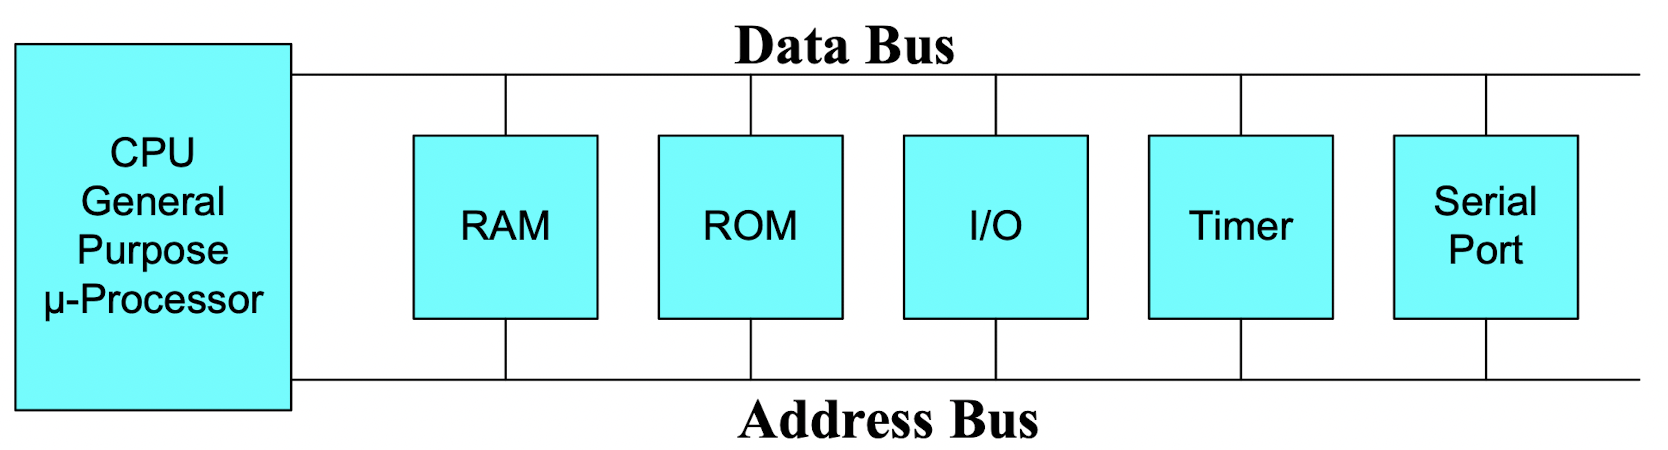
\includegraphics[width=0.9\linewidth]{MPU.png}
          \caption{Microprocessor}
          \label{subfig:MPU.png}
        \end{subfigure}
        \begin{subfigure}[b]{0.3\linewidth}
          \centering
          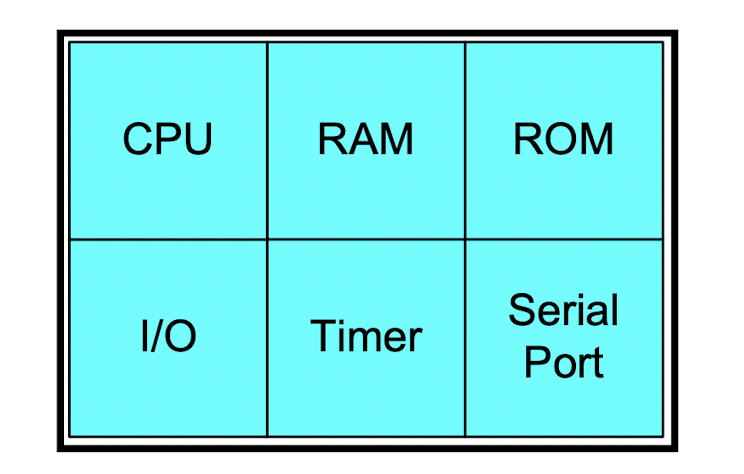
\includegraphics[width=0.9\linewidth]{MCU.png}
          \caption{Microcontroller}
          \label{subfig:MCU.png}
        \end{subfigure}
      \end{figure}

      \begin{table}[H]
        \centering
        \begin{tabular}{p{0.45\linewidth} p{0.45\linewidth}}
          \toprule
          \multicolumn{1}{c}{\textbf{Microprocessor}}                                                                                                             & \multicolumn{1}{c}{\textbf{Micro Controller}}                                                                                                    \\
          \midrule
          Microprocessor is heart of Computer system.                                                                                                             & Micro controller is a hear of embedded system.                                                                                                   \\
          \midrule
          \textbf{It is just a processor. Memory and I/O components have to be connected externally.}                                                             & \textbf{Micro controller has external processor along with internal memory and I/O components.}                                                  \\
          \midrule
          The circuit is large.                                                                                                                                   & The circuit is small.                                                                                                                            \\
          \midrule
          Cannot be used in compact systems and hence inefficient.                                                                                                & Can be used in compact systems and hence it is an efficient technique.                                                                           \\
          \midrule
          Cost of the entire system increases.                                                                                                                    & Cost of the entire system is low.                                                                                                                \\
          \midrule
          Due to external components, the entire power consumption is high. Hence it is not suitable to used with devices running on stored power like batteries. & Since external components are low, total power consumption is less and can be used with devices running on stored power like batteries.          \\
          \midrule
          Most of the microprocessors do not have power saving features.                                                                                          & Most of the micro controllers have power saving modes like idle mode and power saving mode. This helps to reduce power consumption even further. \\
          \midrule
          Since memory and I/O components are all external, each instruction will need external operation, hence it is relatively slower.                         & Since components are internal, most of the operations are internal instruction, hence speed is fast.                                             \\
          \midrule
          Microprocessor have less number of registers, hence more operations are memory based.                                                                   & Micro controller have more number of registers, hence the programs are easier to write                                                           \\
          \midrule
          Microprocessors are based on Von Neumann model/architecture where program and data are stored in same memory module.                                    & Micro controllers are based on Harvard architecture where program memory and Data memory are separate.                                           \\
          \midrule
          Mainly used in personal computers.                                                                                                                      & Used mainly in washing machines, MP2 players.                                                                                                    \\
          \bottomrule
        \end{tabular}
        \label{tab:MCU_MPU}
      \end{table}

    \item \textbf{Von Neumann \& Havard Architecture}
      \begin{figure}[H]
        \centering
        \begin{subfigure}[b]{0.45\linewidth}
          \centering
          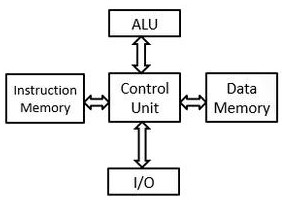
\includegraphics[width=0.9\linewidth]{Harvard_architecture.jpeg}
          \caption{Harvard Architecture}
          \label{subfig:Harvard_architecture.jpeg}
        \end{subfigure}
        \begin{subfigure}[b]{0.45\linewidth}
          \centering
          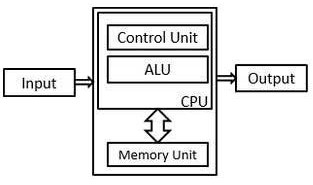
\includegraphics[width=0.9\linewidth]{Von_neumann_architecture.jpeg}
          \caption{Von Neumann Architecture}
          \label{subfig:Von_neumann_architecture.jpeg}
        \end{subfigure}
      \end{figure}

      \begin{table}[H]
        \centering
        \begin{tabular}{p{0.45\linewidth} p{0.45\linewidth}}
          \toprule
          \multicolumn{1}{c}{\textbf{Harvard architecture}}                       & \multicolumn{1}{c}{\textbf{Von Neumann architecture}}                       \\
          \midrule
          \textbf{It required two memories for their instruction and data.}       & \textbf{It required only one memory for their instruction and data.}        \\
          \midrule
          Harvard architecture is required separate bus for instruction and data. & Von Neumann architecture is required only one bus for instruction and data. \\
          \midrule
          Processor can complete an instruction in one cycle                      & Processor needs two clock cycles to complete an instruction.                \\
          \midrule
          Easier to pipeline, so high performance can be achieve.                 & Low performance as compared to Harvard architecture.                        \\
          \midrule
          Comparatively high cost.                                                & It is cheaper.                                                              \\
          \bottomrule
        \end{tabular}
        \label{tab:von_neumann_havard}
      \end{table}
  \end{enumerate}

\section*{L2 --- PIC MCU Architecture}
  \begin{enumerate}[label = \arabic*.]
    \item \textbf{PIC32}
      \begin{figure}[H]
        \centering
        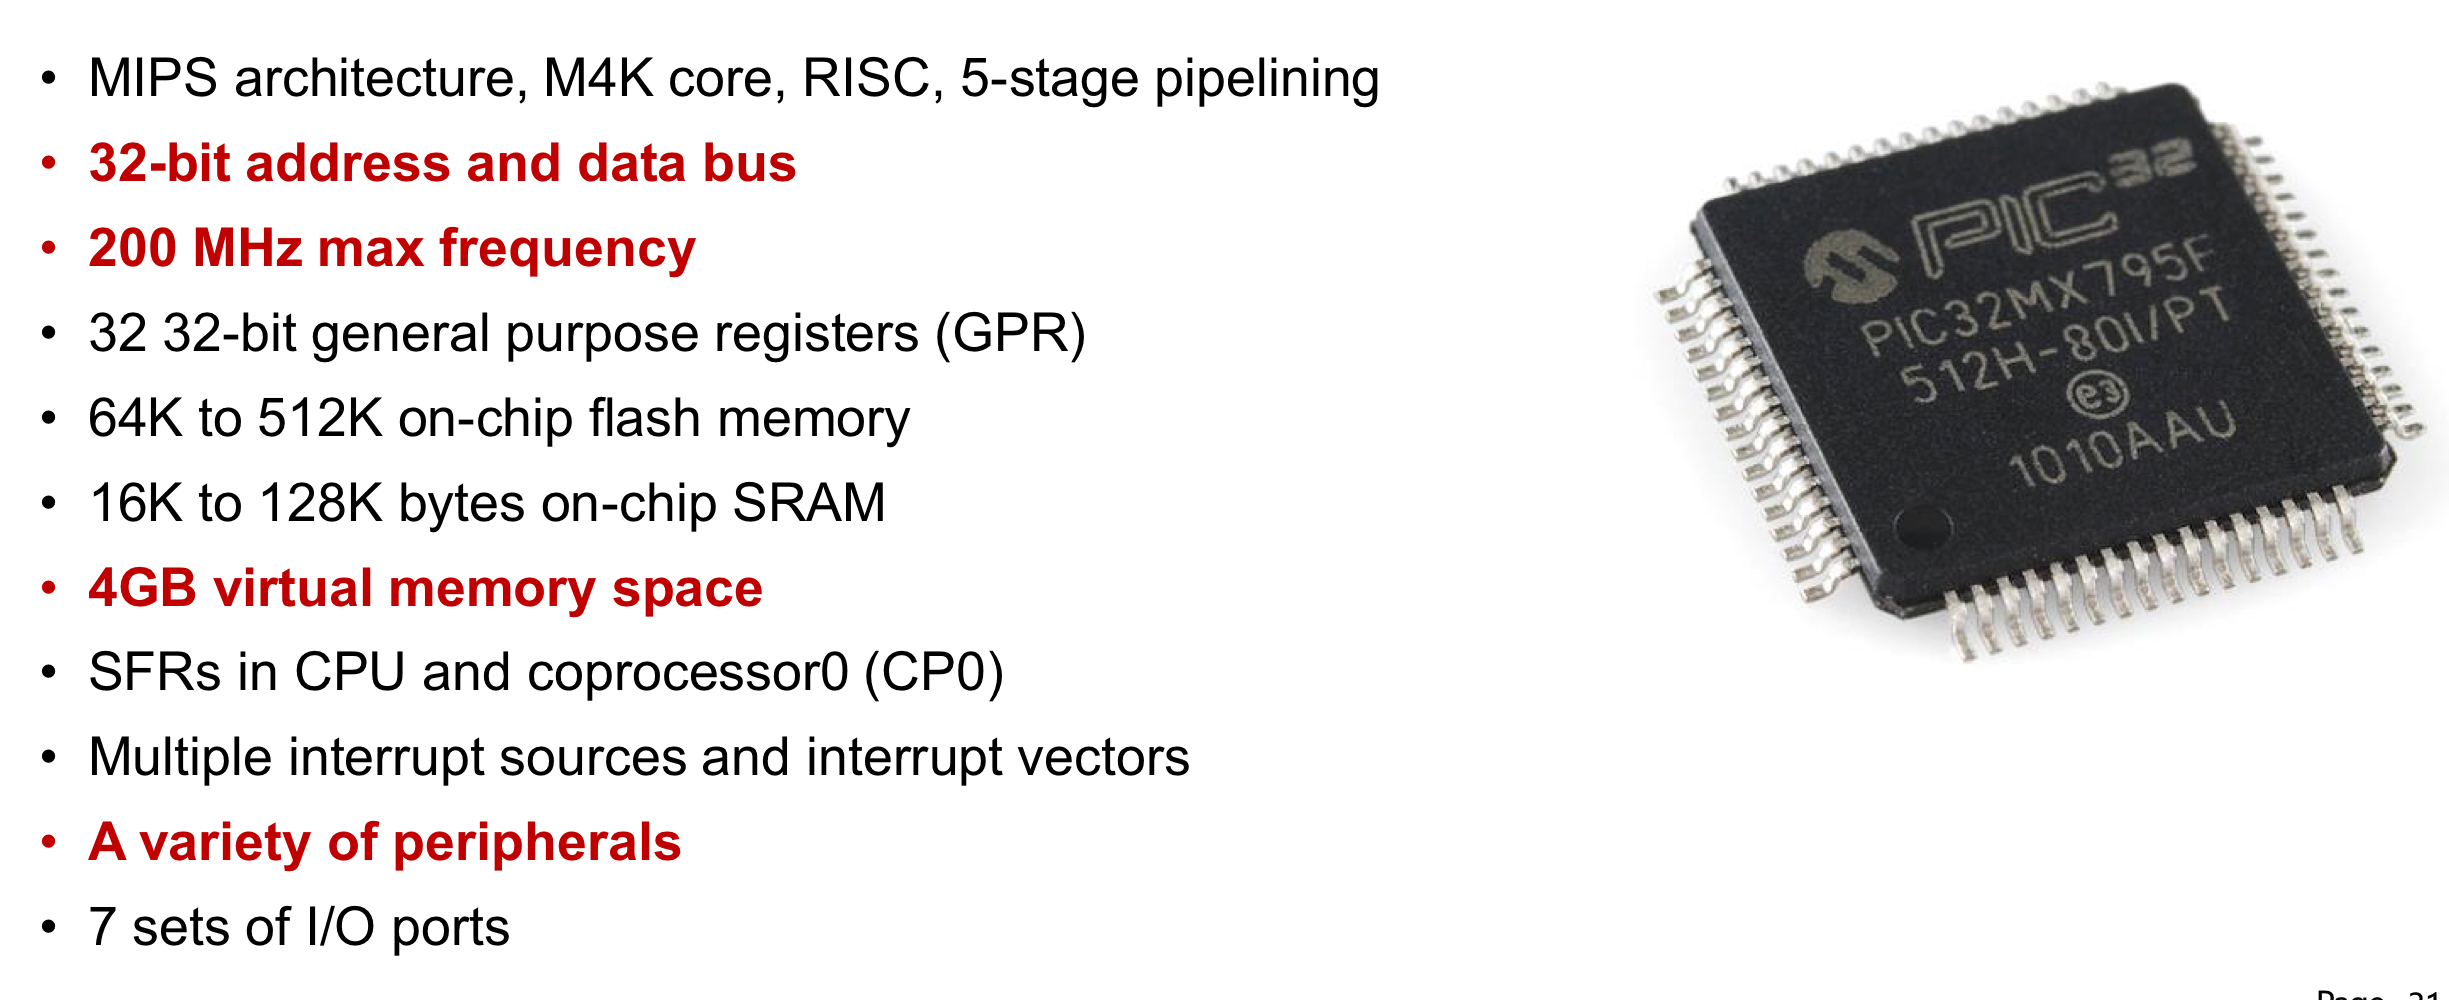
\includegraphics[width=0.9\linewidth]{PIC32_MCU_Architecture_specification.jpeg}
        \caption{32-bit PIC32 MCU Example: Architecture}
        \label{fig:PIC32_MCU_Architecture_specification.jpeg}
      \end{figure}

      \par \( n \)-bit data address bus = support up to \( 2^n \) byte memory.

      \par PIC32 is a combination of Von Neumann and Hasrvard architecture. Harvard architecture on physical falsh memory, and Von Neumann on virtual level and SRAM. See \href{https://blog.flyingpic24.com/2008/10/26/pic32-harvard-or-von-neumann/}{here} for more details if interested.
    \item \textbf{Special Function Register}
      \par Used to config, control and monitor various aspects of the microprocessor's function.
      \par For example, \verb|T1CON|, \verb|TMR1| and \verb|PR1| when using Timer 1.
  \end{enumerate}

\section*{L3 --- Embedded Programming}
  \begin{enumerate}[label = \arabic*.]
    \item \textbf{Compiler}
      \begin{figure}[H]
        \centering
        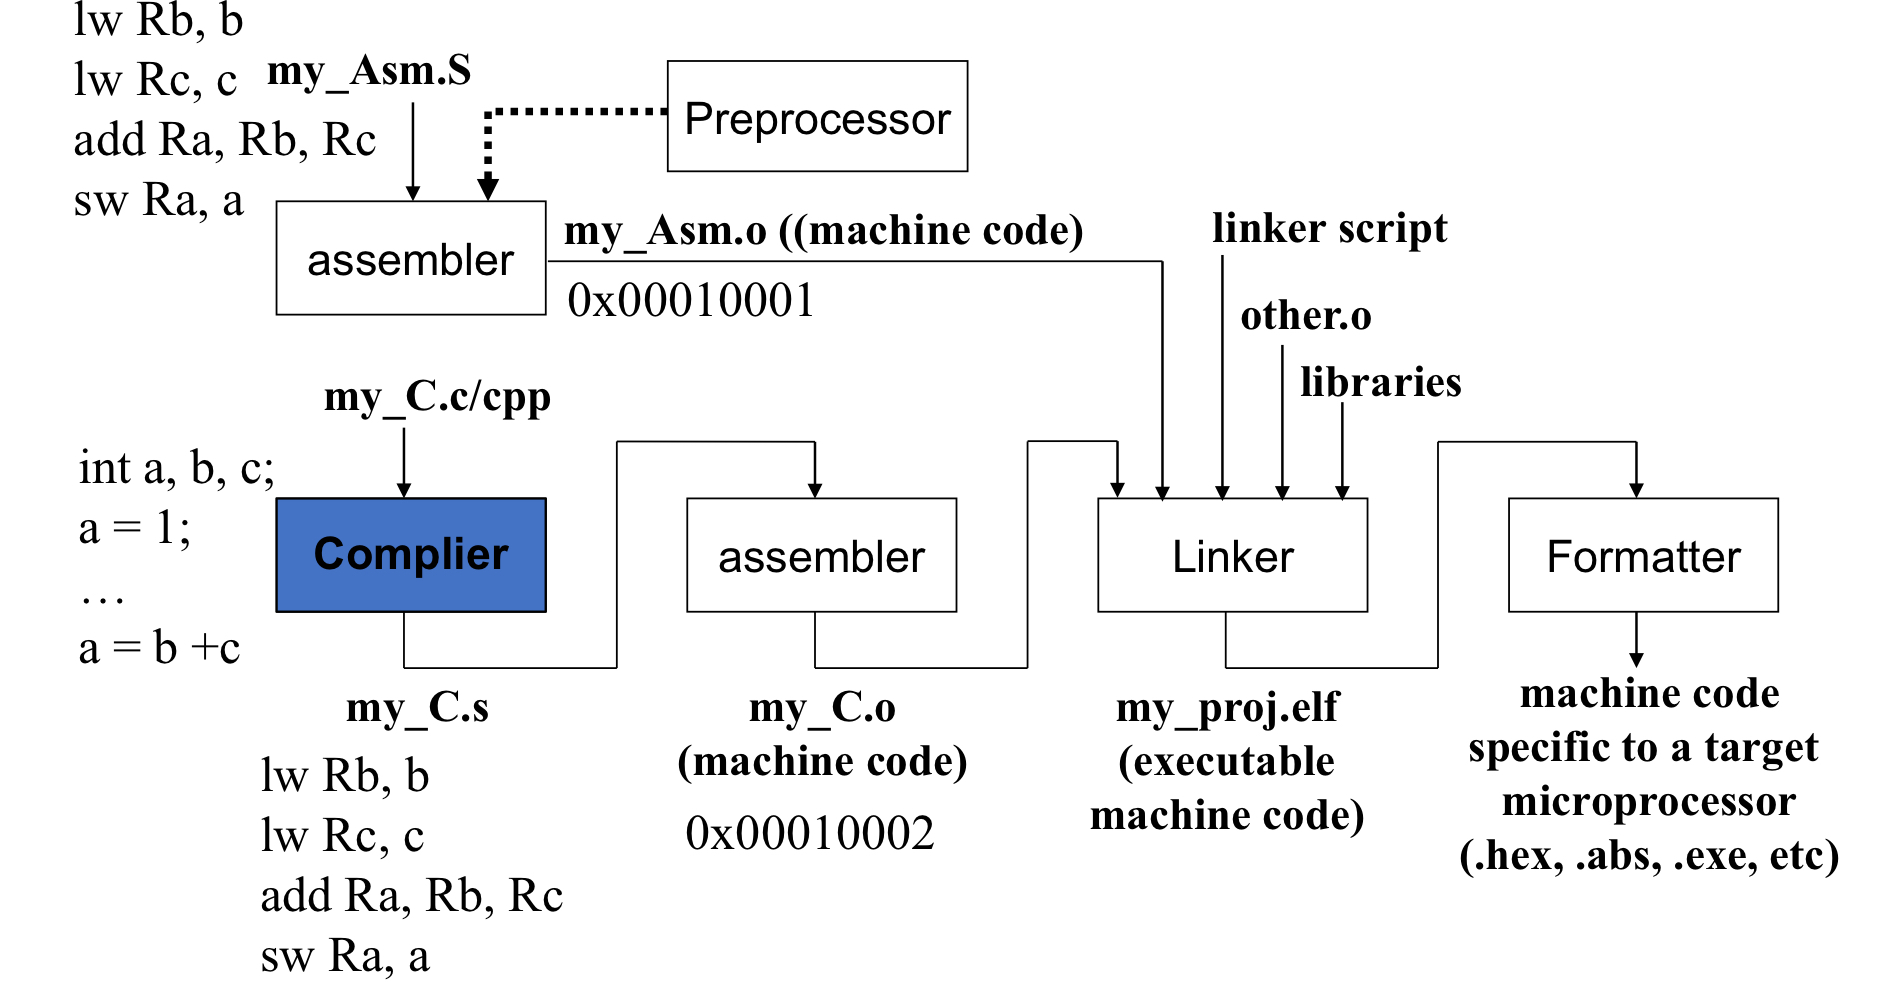
\includegraphics[width=0.9\linewidth]{Program_build_flow.jpeg}
        \caption{Workflow}
        \label{fig:Program_build_flow.jpeg}
      \end{figure}

    \item \textbf{Const \& Volatile}
      \begin{itemize}[leftmargin = 1cm]
        \item const: the value not supposed to be written by program (read only).
        \item volatile: the value can be changed by something other than program so it should be reexamined frequently.
      \end{itemize}
    \item \textbf{Directives}
      \par Directives: compiler dependent commands.
      \par e.g. \verb|#pragma interrupt func_name ipln|.
  \end{enumerate}

\section*{L4 --- Timers and IO}
  \begin{enumerate}[label = \arabic*.]
    \item \textbf{Oscillator}
      \begin{itemize}[leftmargin = 1cm]
        \item \textbf{Internal oscillator}:
          \begin{itemize}[leftmargin = 1cm]
            \item Integrated on-chip within the processor
            \item Low frequency accuracy and stability.
            \item Most of internal oscillator are RC circuits
          \end{itemize}
        \item \textbf{External oscillator}
          \begin{itemize}[leftmargin = 1cm]
            \item Located off-chip on the PCB
            \item High frequency accuracy and stability
            \item Most of external oscillator are crystal oscillator
          \end{itemize}
      \end{itemize}

      \par Peripherals don't have a high clock frequency:
      \begin{itemize}[leftmargin = 1cm]
        \item No need
        \item Limited by parasitics
        \item Power consumption
      \end{itemize}
    \item \textbf{Timer}
      \par Two types, five timers on PIC32:
      \begin{itemize}[leftmargin = 1cm]
        \item Type A --- Timer 1
          \begin{itemize}[leftmargin = 1cm]
            \item \textcolor{red}{16-bit} synchronous/\textcolor{red}{asynchronous} timer/event counter
            \item Internal or external clock source
            \item Gated external event timer
          \end{itemize}
        \item Type B --- Timer 2, 3, 4, 5
          \begin{itemize}[leftmargin = 1cm]
            \item \textcolor{red}{16/32-bit} synchronous timer/event counter
            \item Internal or external clock source
            \item Gated external event timer
          \end{itemize}
      \end{itemize}
      \begin{figure}[H]
        \centering
        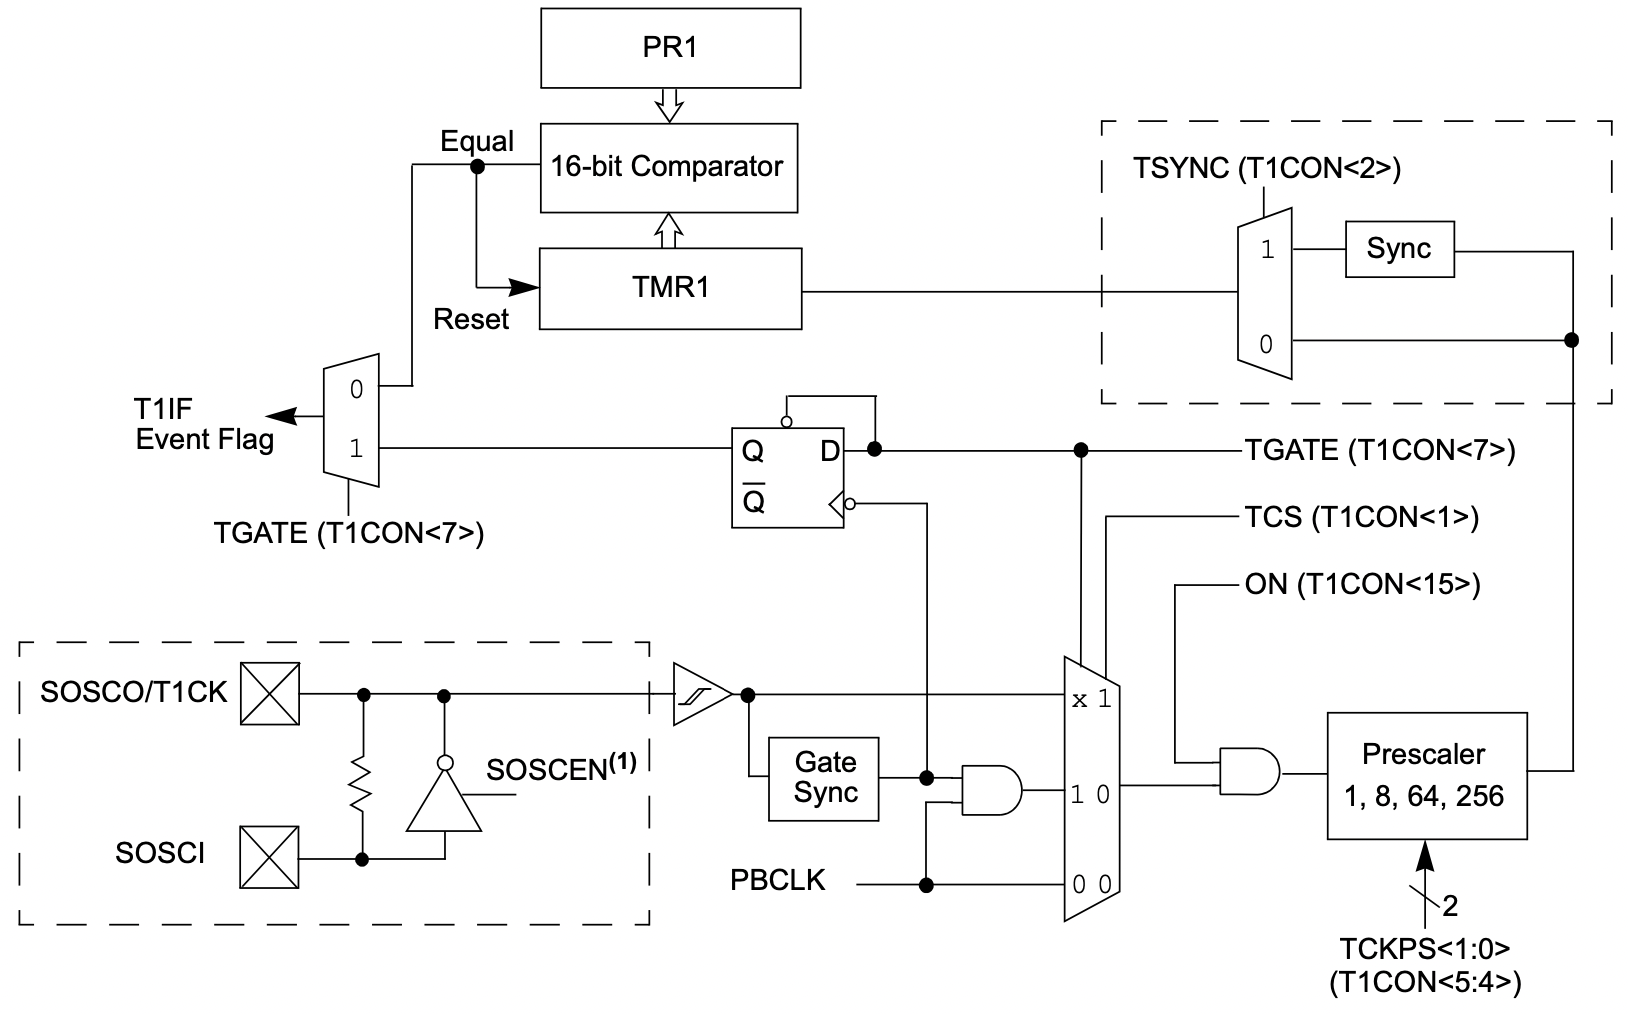
\includegraphics[width=0.9\linewidth]{Timer1_block_diagram.png}
        \caption{Timer 1 block diagram (Datasheet Page.~197)}
        \label{fig:Timer1_block_diagram.png}
      \end{figure}

    \item \textbf{16-bit synchronous timer setup steps}
      \par Use internal clock source --- \verb|PBCLK| as example.
      \begin{enumerate}[label = \arabic*.]
        \item Clear control bit \verb|ON| (\verb|TxCON<15>=0|) to disable timer.
        \item Clear control bit \verb|TCS| (\verb|TxCON<1>=0|) to select internal clock source \verb|PBCLK|.
        \item Select desired clock prescale value.
        \item Load/clear timer register \verb|TMRx| to specify initial counting value.
        \item Load period register \verb|PRx| with desired 16-bit match value.
        \item If interrupts used:
          \begin{enumerate}[label = \roman*.]
            \item Clear interrupt flag bit
            \item Configure interrupt priority and subpriority levels
            \item Set interrupt enable bit
          \end{enumerate}
        \item Set control bit \verb|ON| (\verb|TxCON<15>=1|) to start timer
      \end{enumerate}

  \end{enumerate}

\section*{L4 --- Timers and IO}
  \begin{enumerate}[label = \arabic*.]
    \item \textbf{GPI/O Ports}
      \par Each port has 4 associated registers for its operation:
      \begin{itemize}[leftmargin = 1cm]
        \item \verb|TRISx| register: Data Direction register, or Tri-State Control register
          \begin{itemize}[leftmargin = 1cm]
            \item \verb|1| for input
            \item \verb|0| for output
            \item all port I/O pins are defined as inputs after a device Reset. Certain I/O pins are shared with analog peripherals and default to analog inputs after a device Reset.
          \end{itemize}
        \item \verb|LATx| register: output latch
          \begin{itemize}[leftmargin = 1cm]
            \item used to write date to the port I/O pins. The \verb|LATx| Latch register holds the data written to either
              the \verb|LATx| or \verb|PORTx| registers.
            \item reading the LATx Latch register reads the last value written to the corresponding PORT or Latch register.
          \end{itemize}
        \item \verb|PORTx| register: reads the levels on the pins of the device
          \begin{itemize}[leftmargin = 1cm]
            \item used to read the current state of the signal applied to the port I/O pins
            \item writing to a \verb|PORTx| register performs a write to the port's latch, \verb|LATx| register, latching the data to the port's I/O pins
          \end{itemize}
        \item \verb|ODCx| register: Open-drain control
          \begin{quotation}
            \par Pins are configured as digital outputs by setting the corresponding \verb|TRIS| register bits = 0. When configured as digital outputs, these pins are CMOS drivers or can be configured as open-drain outputs by setting the corresponding bits in the Open-Drain Configuration (\verb|ODCx|) register.
            \par The open-drain feature allows generation of outputs higher than \( V_{DD} \) (e.g., 5V) on any desired 5V tolerant pins by using external pull-up resistors. The maximum open-drain voltage allowed is the same as the maximum \( V_{IH} \) specification.
          \end{quotation}
      \end{itemize}

    \item \cprotect\textbf{\verb|CLR|, \verb|SET| And \verb|INV| Registers}
      \par Provide fast atomic bit manipulations, perform operation in hardware atomically.
      \par Reading SET, CLR and INV registers returns undefined
      values.
      \par E.g. \verb|T2CONSET = 0x8000| in homework 1.
  \end{enumerate}

\section*{L5 --- Interrupts}
  \begin{enumerate}[label = \arabic*.]
    \item \textbf{Detect events}
      \par Dealing with asynchronous events:
      \begin{itemize}[leftmargin = 1cm]
        \item Exceptions caused by program execution
        \item Peripheral needs attention or has completed a requested action
        \item Application makes a system call
      \end{itemize}


    \item \textbf{Software polling}
      \begin{itemize}[leftmargin = 1cm]
        \item We can repeatedly poll the application for peripherals.
        \item When an event occurs, detect this via a poll and take action
        \item Common in small or low-performance real-time embedded systems
          \begin{itemize}[leftmargin = 1cm]
            \item Predictable timing
            \item Low hardware cost
          \end{itemize}
        \item In other systems, wastes CPU time
          \begin{itemize}[leftmargin = 1cm]
            \item Affect processor's responsiveness and efficiency
          \end{itemize}
      \end{itemize}
      \begin{lstlisting}[language=c]
/* Timer control */
T2CON = 0x0;       // Stop Timer2 and clear control register
                   // prescale 1:1, internal clock source
TMR2 = 0x0;        // Clear Timer
PR2 = 0xFFFF;
T2CONSET = 0x8000; //Start Timer2

/* polling */
while (TMR2 != 1000);

/* move on */
...
      \end{lstlisting}
    \item \textbf{Interrupt}
      \begin{itemize}[leftmargin = 1cm]
        \item Let the application for peripheral notify us automatically.
        \item Take action (respond to the event) when such a notification occurs (or shortly later).
      \end{itemize}

      \par When a special event or error occurs
      \begin{itemize}[leftmargin = 1cm]
        \item I/O controller interrupts CPU -- by a call from the I/O hardware
        \item CPU stops executing the current program
        \item CPU goes to run an \textbf{interrupt handler} (a special piece of program) or \textbf{interrupt service routine} (ISR)
        \item After finish executing the ISR, CPU returns back to the interrupted program and resume
        \item Not synchronized to instruction execution, may happen between any two instructions
      \end{itemize}
    \item \textbf{Typical Types of Interrupts}
      \begin{itemize}[leftmargin = 1cm]
        \item Internal (exception)
          \begin{itemize}[leftmargin = 1cm]
            \item By CPU errors
            \item By bad instructions
          \end{itemize}
        \item External (interrupt)
          \begin{itemize}[leftmargin = 1cm]
            \item External I/O device
            \item Timer
            \item Reset
            \item System failure
          \end{itemize}
      \end{itemize}
      \par Interrupt comes as a high-level signal or a rising edge depending on processors

    \item \textbf{SFRs for Interrupt}
      \begin{itemize}[leftmargin = 1cm]
        \item \verb|INTCON| -- Interrupt Control Register
        \item \verb|INTSTAT| -- Interrupt Status Register
        \item \verb|TPTMR| -- Temporal Proximity Timer Register
        \item \verb|IFSx| -- Interrupt Flag Status Registers
        \item \verb|IECx| -- Interrupt Enable Control Registers
        \item \verb|IPCx| -- Interrupt Priority Control Registers
      \end{itemize}

    \item \textbf{Interrupt Control}
      \begin{enumerate}[label = \arabic*.]
        \item Enable interrupt globally
        \item Config \verb|INTCON| to select multi vector mode.
        \item Enable individual interrupt, set priority
        \item When interrupt event happens, flag is set regardless of the enable bit
        \item If enabled, interrupt service routine (ISR)
        \item In ISR, service interrupt, clear interrupt flag (for most interrupt requests)
        \item Main program resumes
      \end{enumerate}

    \item \textbf{Enable/disable all interrupt sources globally}
      \begin{itemize}[leftmargin = 1cm]
        \item \verb|asm("ei"); // inline MIPS32 assembly|
        \item \verb|asm("di");|
        \item Corresponding to enable/disable IE bit (\verb|STATUS<0>|)
        \item Must be enabled before individual interrupt can be used
      \end{itemize}

    \item \textbf{Operation Mode}
      \begin{itemize}[leftmargin = 1cm]
        \item Controlled by \verb|MVEC| bit in \verb|INTCON|
        \item \textbf{Single vector mode:}
          \begin{itemize}[leftmargin = 1cm]
            \item All interrupt requests will be serviced at one vector address (default upon reset)
            \item One location for all different interrupts
            \item have to determine what exception/interrupt has just happened, by checking status registers
            \item \verb|if...else...| structure
          \end{itemize}
        \item \textbf{Multi vector mode:} Interrupt requests will be serviced at the calculated vector address
          \begin{itemize}[leftmargin = 1cm]
            \item One location for one (or a small number of) interrupt
            \item Take actions or handle interrupts directly
          \end{itemize}
      \end{itemize}

    \item \textbf{Interrupt Vector Table}
      \begin{figure}[H]
        \centering
        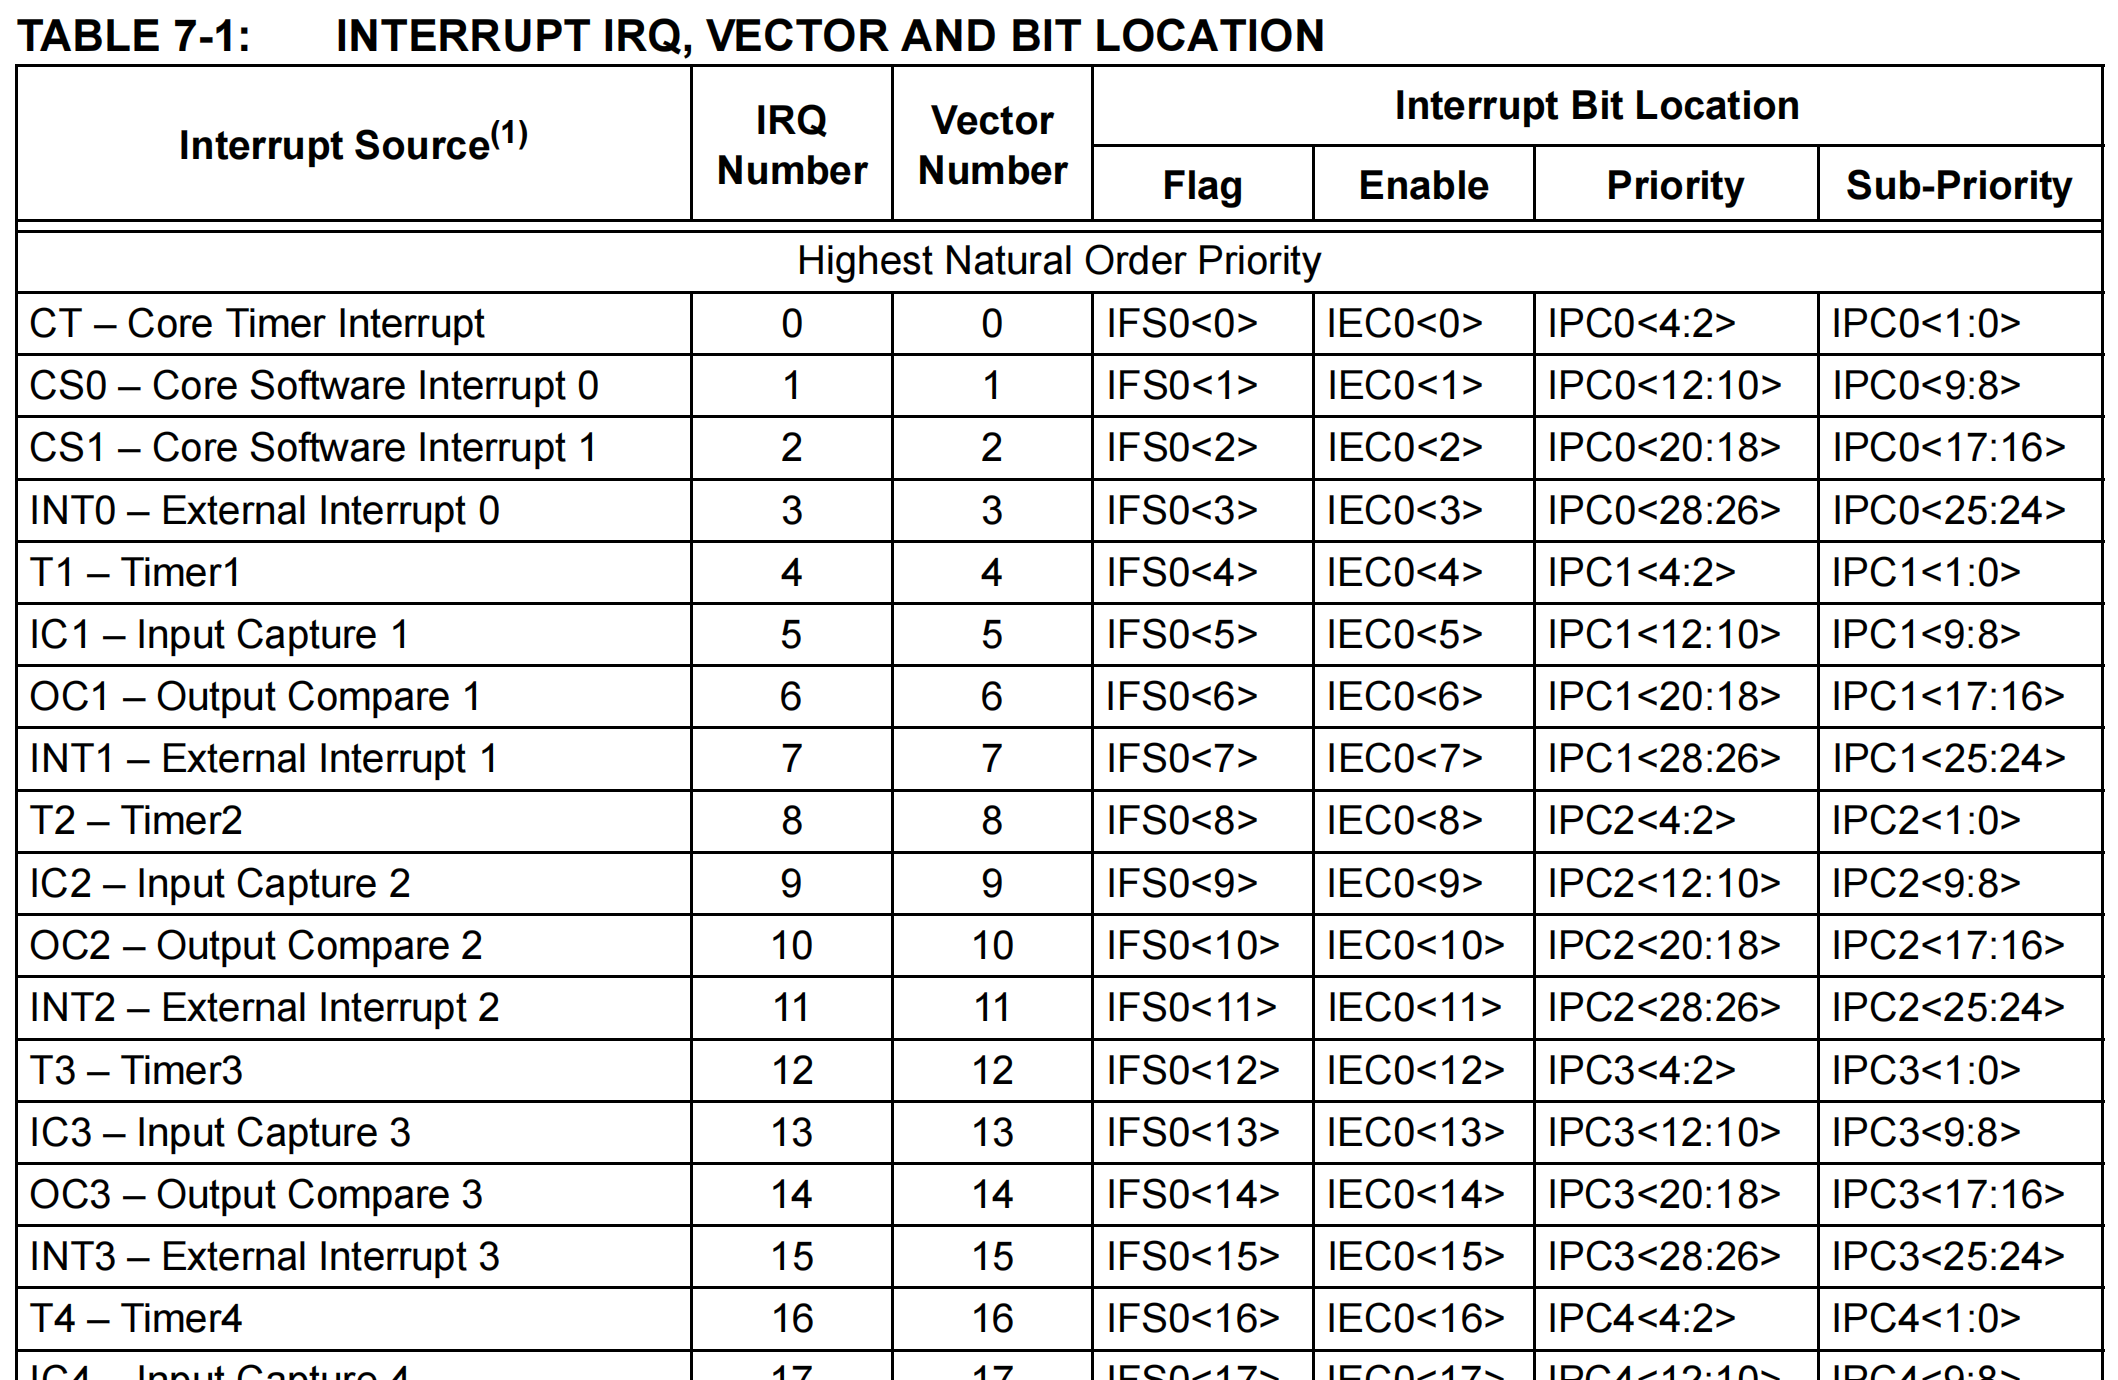
\includegraphics[width=0.9\linewidth]{Interrupt_table.png}
        \label{fig:Interrupt_table.png}
      \end{figure}

    \item \textbf{ISR --- Interrupt Service Routine}
      \par Interrupt flag should be cleared in ISR\@. Otherwise interrupt will be triggered over and over again.

      \par In ISR, you need to
      \begin{itemize}[leftmargin = 1cm]
        \item Clear interrupt flag
        \item Perhaps, stop peripheral
        \item Perhaps, disable interrupt (if in critical section)
        \item Do whatever you need to do, fix problem, respond to the peripheral
        \item Perhaps, some configuration
        \item Perhaps, restart peripheral for next interrupt
        \item Perhaps, re-enable interrupt
        \item Perhaps, start another peripheral for another interrupt
        \item Return to the interrupted instruction
      \end{itemize}

    \item \textbf{Critical section/region}
      \par Should NOT be interrupted
      \par Should disable interrupts while executing those instructions

    \item \textbf{Interrupt priority}
      \par Devices needing more urgent attention get higher priority
      \par Higher priority interrupt can interrupt execution of a lower priority interrupt

      \par Three priority levels
      \begin{itemize}[leftmargin = 1cm]
        \item Group level: 0 - 7 (highest)
        \item Subgroup level: 0 - 3 (highest)
        \item Natural level: 0 - 63 (lowest)
      \end{itemize}

    \item \textbf{Preemption}
      \par Higher priority interrupt request (IRQ) preempts (overrides) any lower priority interrupts (on group level).
      \par No preemption on subgroup and natural levels.

    \item \textbf{IPL and RIPL}
      \begin{itemize}[leftmargin = 1cm]
        \item Requested interrupt priority level (RIPL)
          \begin{itemize}[leftmargin = 1cm]
            \item In field \verb|RIPL| (\verb|CAUSE<12:10>|)
            \item 0\ldots 7, encode requested interrupt priority
          \end{itemize}
        \item Current CPU priority (IPL)
          \begin{itemize}[leftmargin = 1cm]
            \item In field \verb|IPL| (\verb|STATUS<12:10>|)
            \item Usually default 0 (no interrupt), changes to IRQ priority when servicing IRQ
            \item 0\ldots 7, encode the MIPS interrupt priority hierarchy
          \end{itemize}
        \item Preemption happens only when \verb|RIPL| \( > \) \verb|IPL|
      \end{itemize}

    \item \textbf{How to write ISR}
      \begin{lstlisting}[language = c]
#pragma interrupt foo ipl4 vector @23
void foo(void){
  ...
}
// foo will be located at the address of interrupt vector 23

#pragma interrupt bar ipl5 vector 23
void bar(void){
  ...
}
// bar will be located in general purpose program memory
// A dispatch function targeting bar will be created at exception vector address 23
    \end{lstlisting}
      \par \verb|iplx|, \verb|x| = 0\ldots 7, 0 means interrupt disabled. \verb|x| must match the group interrupt priority level specified in \verb|IPCx.|
      \par Each interrupt vector has 8 words, usually holding dispatch function that associates the vector address with the real interrupt handler function.

    \item \textbf{Change Notice (CN)}
      \par Generate interrupt upon change of state on selected CN pins
      \begin{itemize}[leftmargin = 1cm]
        \item CN pins must be configured as inputs
        \item Two adjacent reads (delayed by \verb|SYSCLK|) of CN PORT are compared, mismatch generated if different
        \item Any mismatch provides an interrupt signal
      \end{itemize}
    \item \textbf{CN configuration}
      \begin{enumerate}[label = \arabic*.]
        \item Disable all interrupts
        \item Set selected CN pin as input
        \item Enable CN module (\verb|CNCON.ON = 1|)
        \item Enable individual CN inputs, and pull ups (optional)
        \item \textcolor{magenta}{Read corresponding PORT registers to clear pre-existing mismatch condition}
        \item Configure the CN interrupt priority
        \item Clear CN interrupt flag
        \item Enable CN interrupt
        \item Enable all interrupts
      \end{enumerate}

    \item \textbf{CN ISR}
      \begin{enumerate}[label = \arabic*.]
        \item Temporarily disable CN interrupt
        \item \textcolor{magenta}{PORT should be read to clear mismatch condition}
        \item Interrupt flag should be cleared by user program
        \item \textcolor{magenta}{Current PORT value should be compared with the last PORT value of the same pin to determine which CN pin changed}
        \item Re-enable CN interrupt
      \end{enumerate}

      \par Note:
      \begin{enumerate}[label = \arabic*.]
        \item CN interrupt is a persistent interrupt: only clearing IF flag is not enough, must clear the corresponding condition.
        \item CN interrupts of all pins go into the same vector address (vector number 26). Therefore in ISR we should check which IO pin is changed.
      \end{enumerate}


  \end{enumerate}

\section*{L6 --- Liquid-Crystal Display (LCD) Driver}
  \begin{enumerate}[label = \arabic*.]
    \item \textbf{Make good use of datasheet}
      \par The datasheet of LCD is file \verb|lcd1602a_398762.pdf| in \verb|./Reference_Materials/PIC32 Starter Kit/|.

    \item \textbf{LCD module}
      \begin{figure}[H]
        \centering
        \begin{subfigure}[b]{0.6\linewidth}
          \centering
          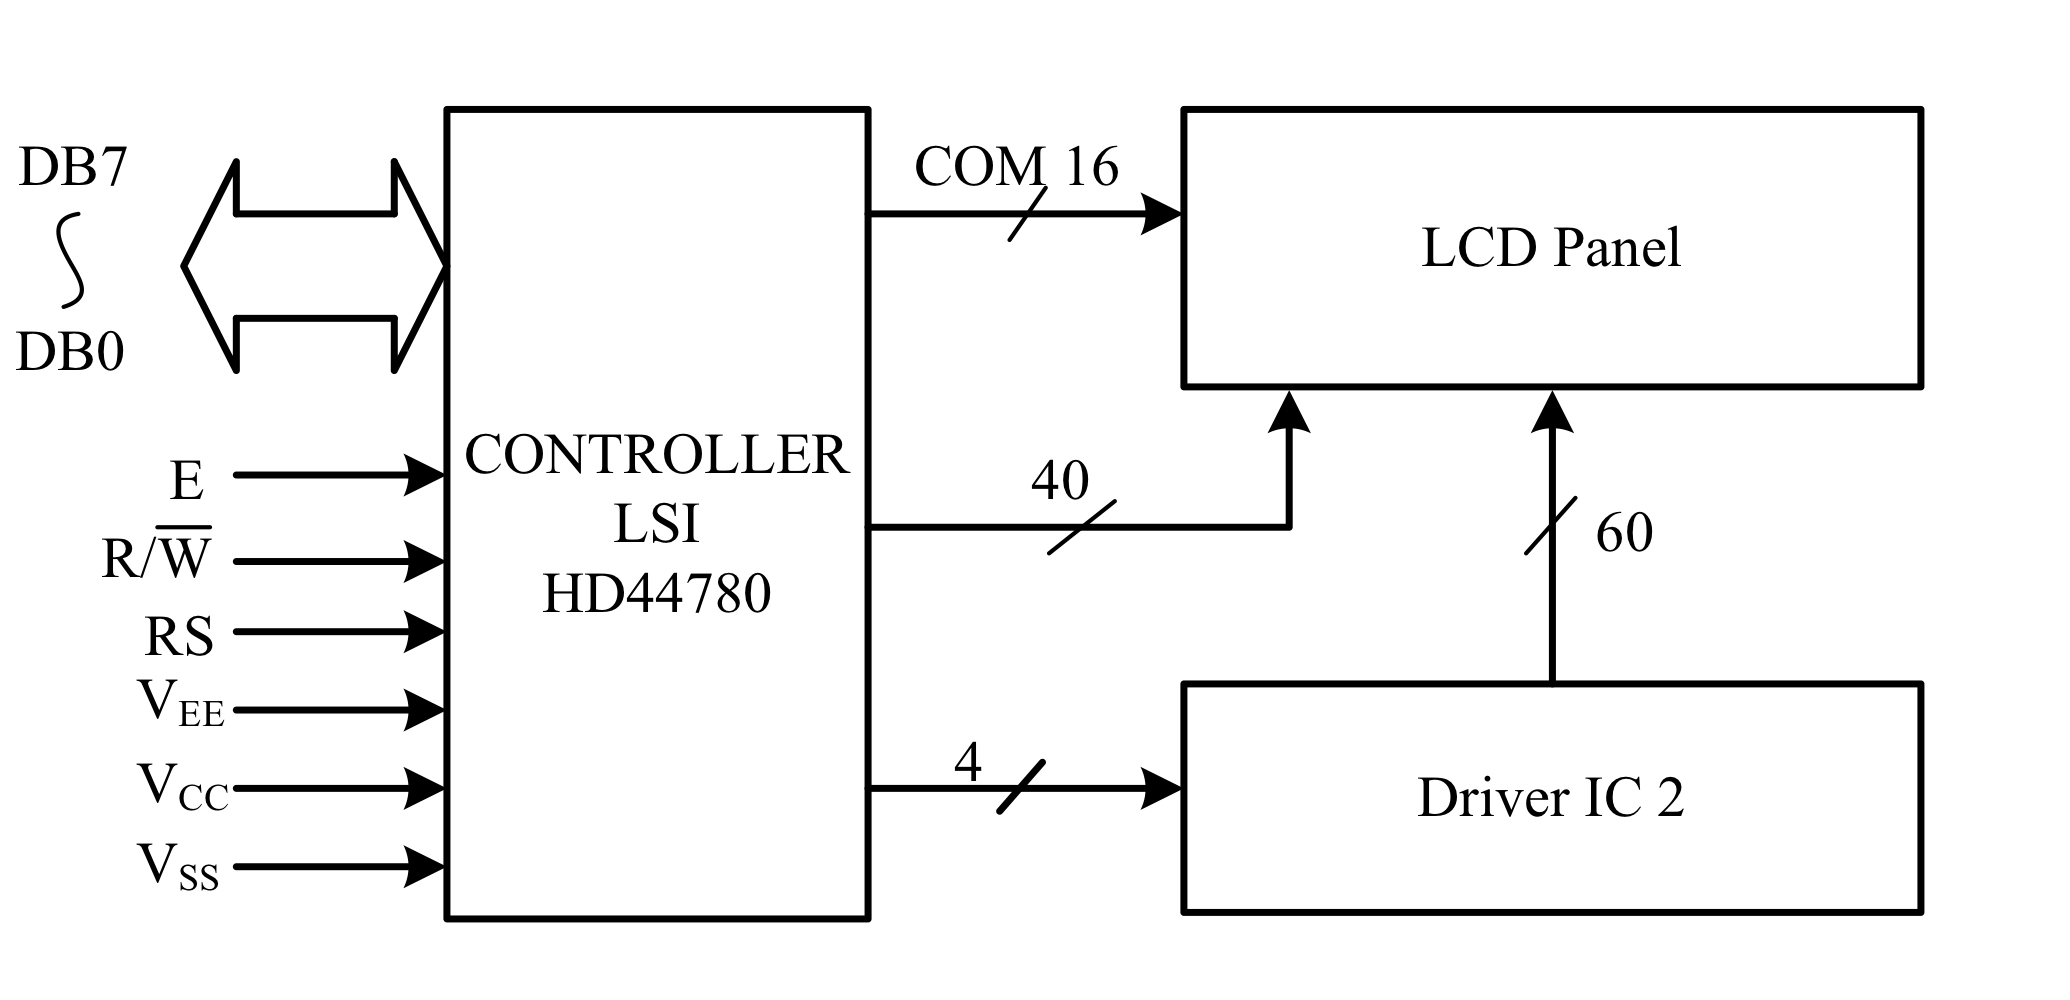
\includegraphics[width=0.9\linewidth]{LCD_module.jpeg}
          \caption{LCD module}
          \label{subfig:LCD_module.jpeg}
        \end{subfigure}
        \begin{subfigure}[b]{0.3\linewidth}
          \centering
          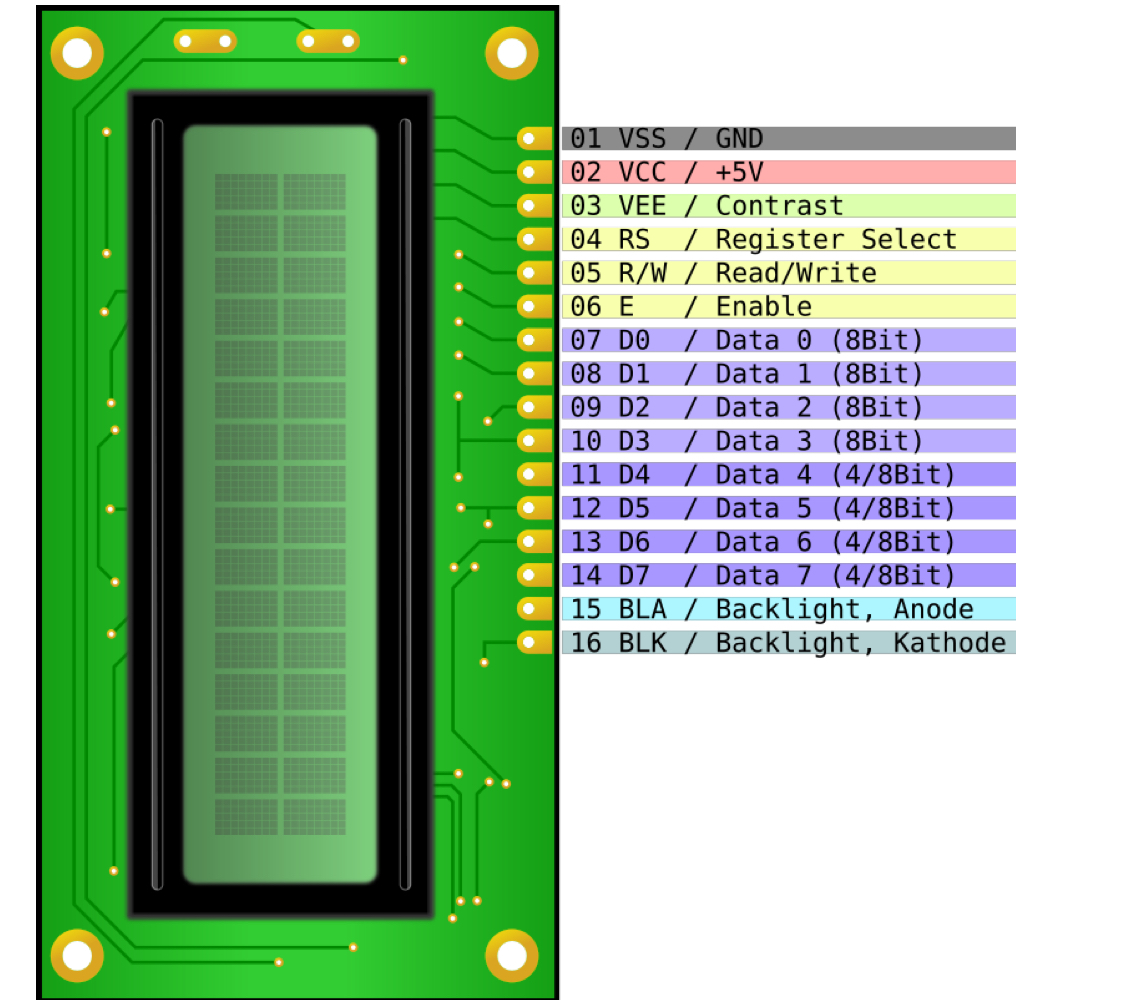
\includegraphics[width=0.9\linewidth]{LCD_pins_definition.jpeg}
          \caption{LCD pins definition}
          \label{subfig:LCD_pins_definition.jpeg}
        \end{subfigure}
        \label{fig:LCD_module}
      \end{figure}

    \item \textbf{Display Data RAM (DDRAM)}
      \begin{itemize}[leftmargin = 1cm]
        \item Can hold up to 80 bytes (characters)
        \item 40 locations mapped to Line1: \verb|0x00 - 0x27|
        \item 40 locations mapped to Line2: \verb|0x40 - 0x67|
        \item 2 line \( \times \) 16 display window is aligned with DDRAM from the head
          \begin{figure}[H]
            \centering
            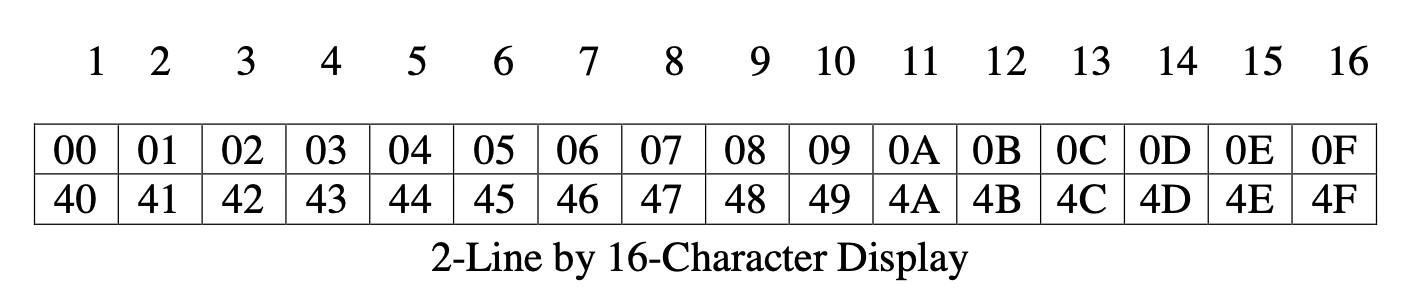
\includegraphics[width=0.6\linewidth]{Display_window.png}
            \label{fig:Display_window.png}
          \end{figure}
        \item Display window can be shifted left or right
      \end{itemize}

    \item \textbf{Code Generate ROM (CGROM)}
      \par It can be understood as the 8-bit encoding of actual character patterns. Almost the same as ASCII chart except some characters.

    \item \textbf{Control Inputs}
      \begin{itemize}[leftmargin = 1cm]
        \item RS, R/W
          \begin{figure}[H]
            \centering
            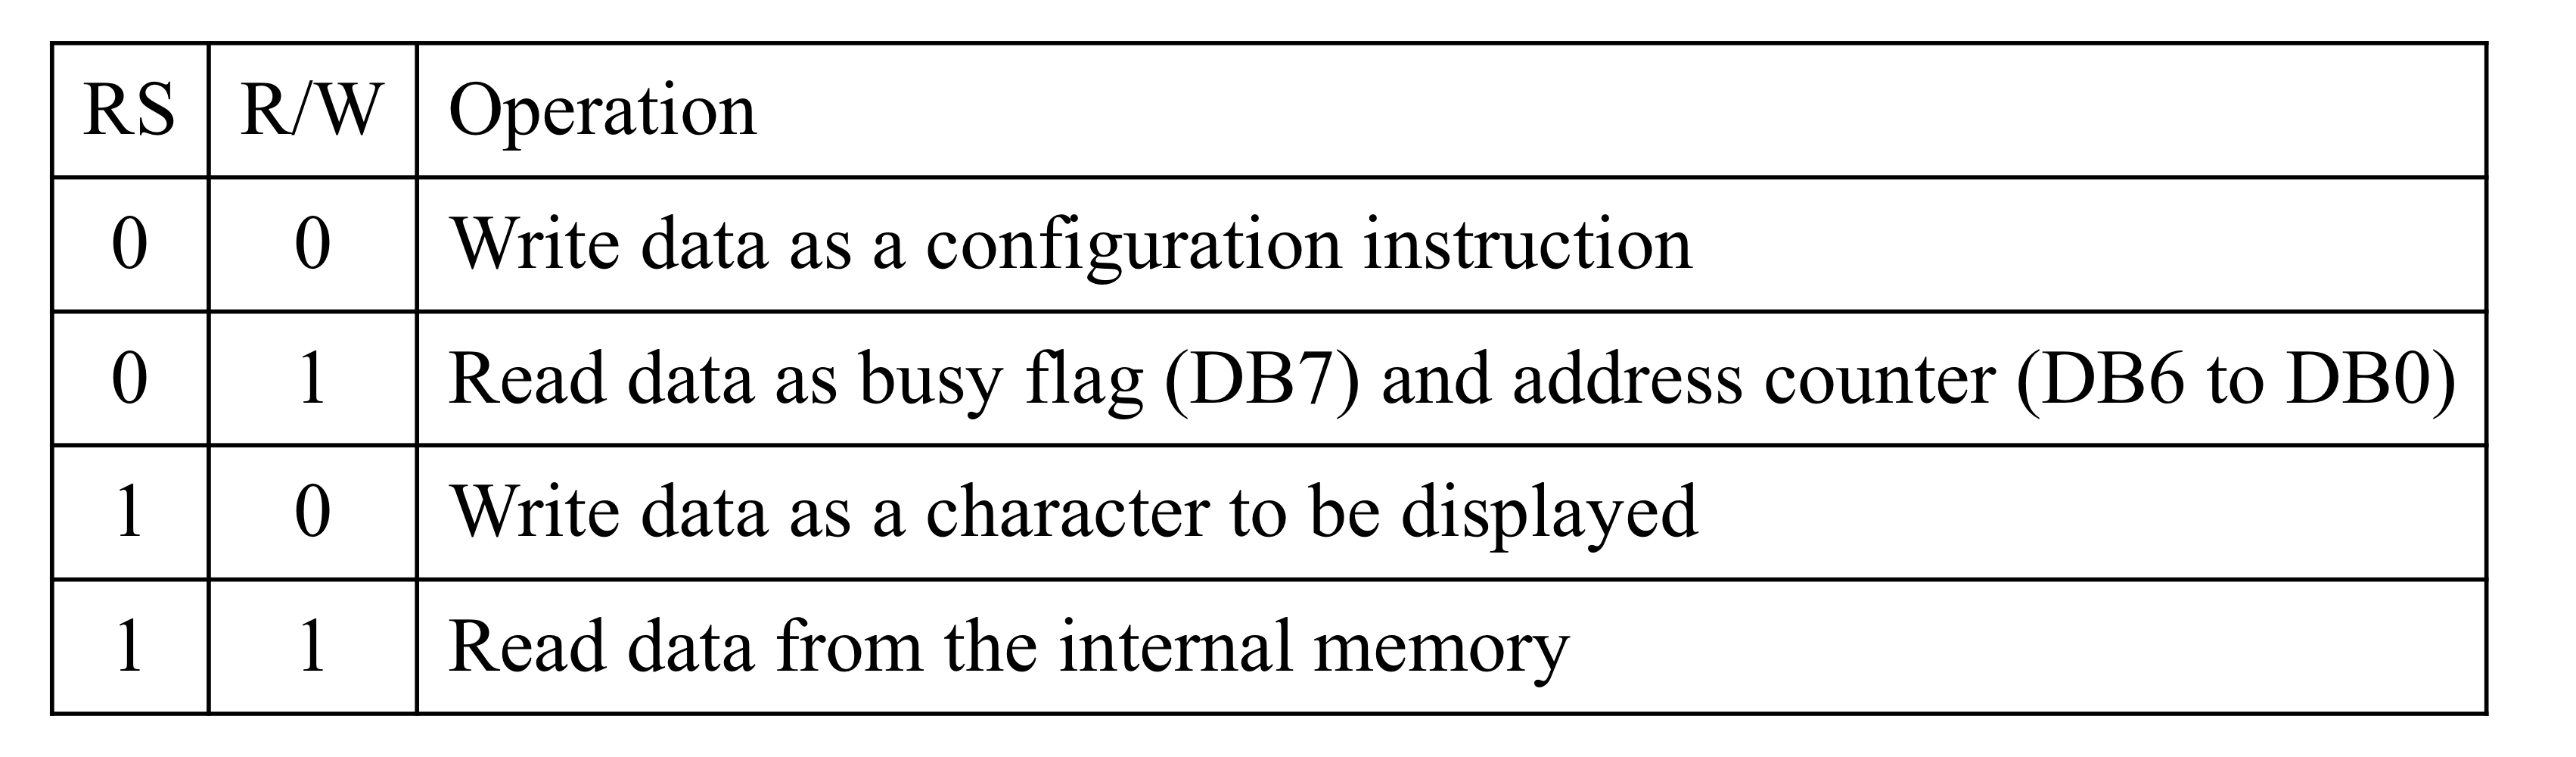
\includegraphics[width=0.6\linewidth]{RS_RW_definition.jpeg}
            \label{fig:RS_RW_definition.jpeg}
          \end{figure}
        \item E -- data transfer enable
          \par a High to Low transition on E enables the data transfer
      \end{itemize}

    \item \textbf{Instruction table}
      \par Defines the inputs to perform specific instruction. Refer to the datasheet.

    \item \textbf{Timing requirements}
      \begin{itemize}[leftmargin = 1cm]
        \item Important, must be satisfied.
        \item All instruction execution time must be satisfied, except
          \begin{itemize}[leftmargin = 1cm]
            \item For 4-bit interface, two consecutive writes, one for high nibble, one for low nibble, need no delay in between, but need 40 \( \mu \)sec after
            \item read instruction needs no time
          \end{itemize}
        \item Each write operation is enabled by a high to low transition on E input
          \par including the two consecutive nibble write
      \end{itemize}

    \item \textbf{Initialization}
      \begin{figure}[H]
        \centering
        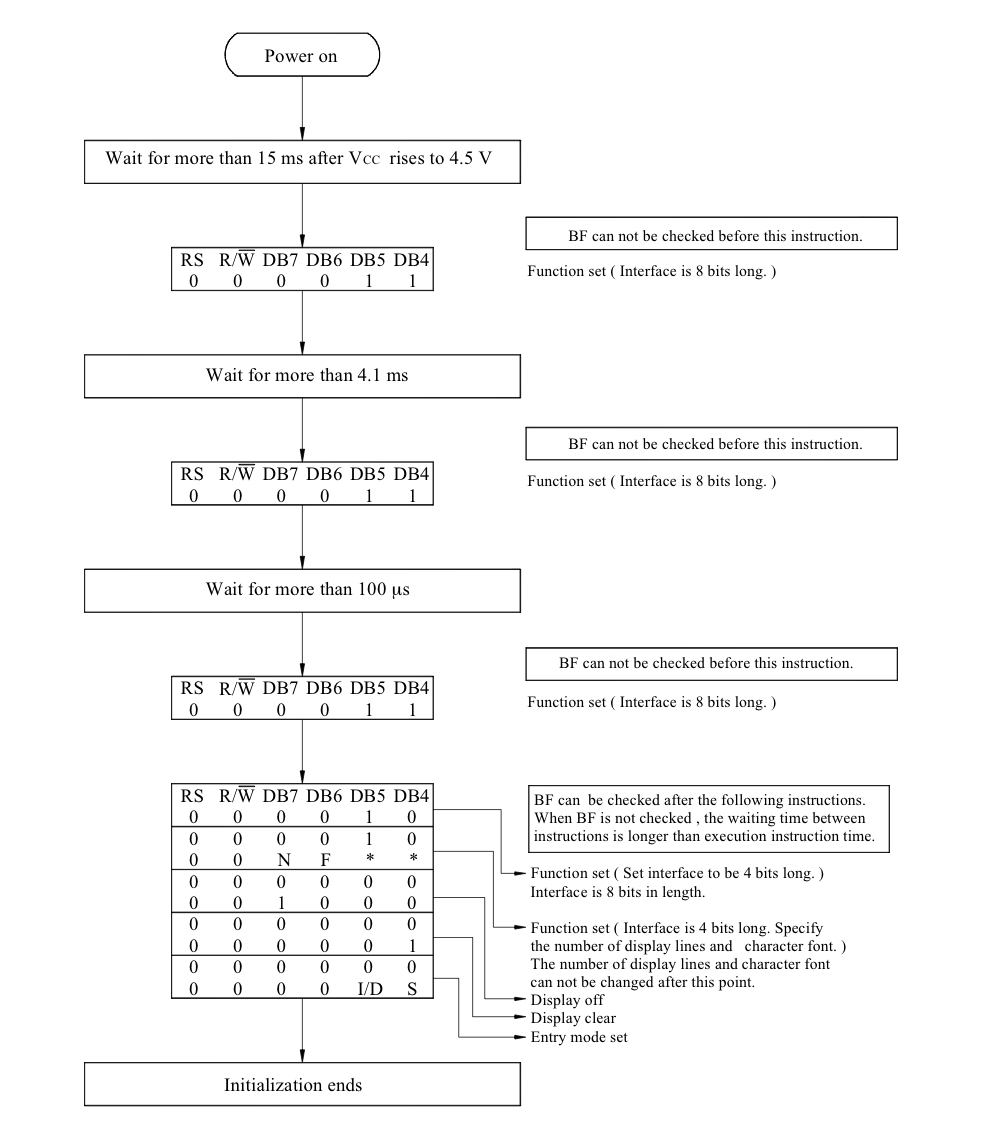
\includegraphics[width=0.9\linewidth]{LCD_config_4bit_step.jpeg}
        \caption{LCD 4-bit interface initialization}
        \label{fig:LCD_config_4bit_step.jpeg}
      \end{figure}

  \end{enumerate}

\section*{L7 --- Power-saving Operations}
  \begin{enumerate}[label = \arabic*.]
    \item \textbf{Static/Dynamic power}
      \par Dynamic power is comprised of switching and short-circuit power.
      \par Static power is comprised of leakage, or current that flows through the transistor when there is no activity.
      \begin{equation*}
        \begin{aligned}
          P_{\text{dynamic}} & = C V^2 f             \\
          P_{\text{static}}  & = V I_{\text{static}} \\
        \end{aligned}
      \end{equation*}

    \item \textbf{Reduce power consumption}
      \begin{itemize}[leftmargin = 1cm]
        \item Reduce operation frequency (lower frequency, lower power consumption)
        \item Halt CPU or disable peripheral modules
      \end{itemize}

    \item \textbf{9 power saving modes}
      \begin{itemize}[leftmargin = 1cm]
        \item CPU running
          \begin{itemize}[leftmargin = 1cm]
            \item FRC RUN mode: CPU uses \verb|FRC| clock source
            \item LPRC RUN mode: CPU uses \verb|LPRC| clock source
            \item SOSC RUN mode: CPU uses \verb|SOSC| clock source
            \item Peripheral bus scaling mode: \verb|PBCLK| is fraction of \verb|SYSCLK|
          \end{itemize}

        \item CPU halted
          \begin{itemize}[leftmargin = 1cm]
            \item SLEEP mode: anything using \verb|SYSCLK| (CPU and peripherals) halted, peripheral using other clock source are operating – lowest power consumption
            \item POSC IDLE mode: Primary Oscillator
            \item FRC IDLE mode: Fast RC Oscillator (8 MHz)
            \item LPRC IDLE mode: Low-Power RC Oscillator (32 KHz)
            \item SOSC IDLE mode: Secondary Oscillator (32.768 KHz)
          \end{itemize}
      \end{itemize}

    \item \textbf{SLEEP mode}
      \begin{itemize}[leftmargin = 1cm]
        \item Characteristics
          \par CPU and most peripherals are halted
          \par System clock source is shut down
          \par Lowest power consumption
          \par Several peripherals alive to wake up CPU
        \item Enter SLEEP mode
          \par \verb|SLPEN| (\verb|OSCCON<4>|) bit set, followed by “wait” assembly instruction
        \item Exit sleep mode (wake up)
          \par By these events
          \begin{itemize}[leftmargin = 1cm]
            \item Interrupt from operating peripheral
            \item Watch dog timer
            \item Reset
          \end{itemize}
          \par \textcolor{magenta}{May need start-up delay}
          \begin{itemize}[leftmargin = 1cm]
            \item Program not start running until clock signal detected stable
            \item May report fail if delay is too long
          \end{itemize}
        \item Example
          \begin{lstlisting}[language=c]
SYSKEY = 0x0;            // Write invalid key to force lock
SYSKEY=0xAA996655;       // write Key1 to SYSKEY
SYSKEY=0x556699AA;       // Write Key2 to SYSKEY
OSCCONSET = 0x10;        // Set power-saving mode as SLEEP
SYSKEY = 0x0;            // Write invalid key to force lock

asm volatile ("wait");   // Put device in selected power-saving mode
                         // code execution will resume here after
                         // wake and the ISR is complete.
                         // "volatile" forces instruction location in
                         // the program

...user code after wake-up...
        \end{lstlisting}
      \end{itemize}

    \item \textbf{IDLE mode}
      \begin{itemize}[leftmargin = 1cm]
        \item CPU is halted
          \begin{itemize}[leftmargin = 1cm]
            \item System clock source is still running
            \item Peripherals alive, unless individually configured to halt when in IDLE
            \item \textcolor{magenta}{Low start-up latency}
            \item Operating clock frequency may be slowed down to reduce power consumption
          \end{itemize}
        \item Enter IDLE mode
          \par \verb|SLPEN| (\verb|OSCCON<4>|) bit cleared followed by “wait” assembly instruction, e.g.  \\
          \verb|OSCCONCLR = 0x10; asm ("wait");|
        \item Exit from IDLE mode
          \begin{itemize}[leftmargin = 1cm]
            \item Interrupt from operating peripheral
            \item Watch dog timer
            \item Reset
          \end{itemize}
      \end{itemize}

    \item \textbf{Wake-up CPU}
      \begin{itemize}[leftmargin = 1cm]
        \item Peripheral interrupt
          \begin{itemize}[leftmargin = 1cm]
            \item If current CPU priority is greater (IPL \( > \) RIPL), CPU remains halted
              \par System remains IDLE, or system enters IDLE from SLEEP
            \item If requested peripheral IRQ priority is greater (RIPL \( > \) IPL)
              \par CPU services IRQ, then continues executing instruction following “wait”
          \end{itemize}

        \item WDT (watch dog timer) Non-Maskable Interrupt (NMI)
          \begin{figure}[H]
            \centering
            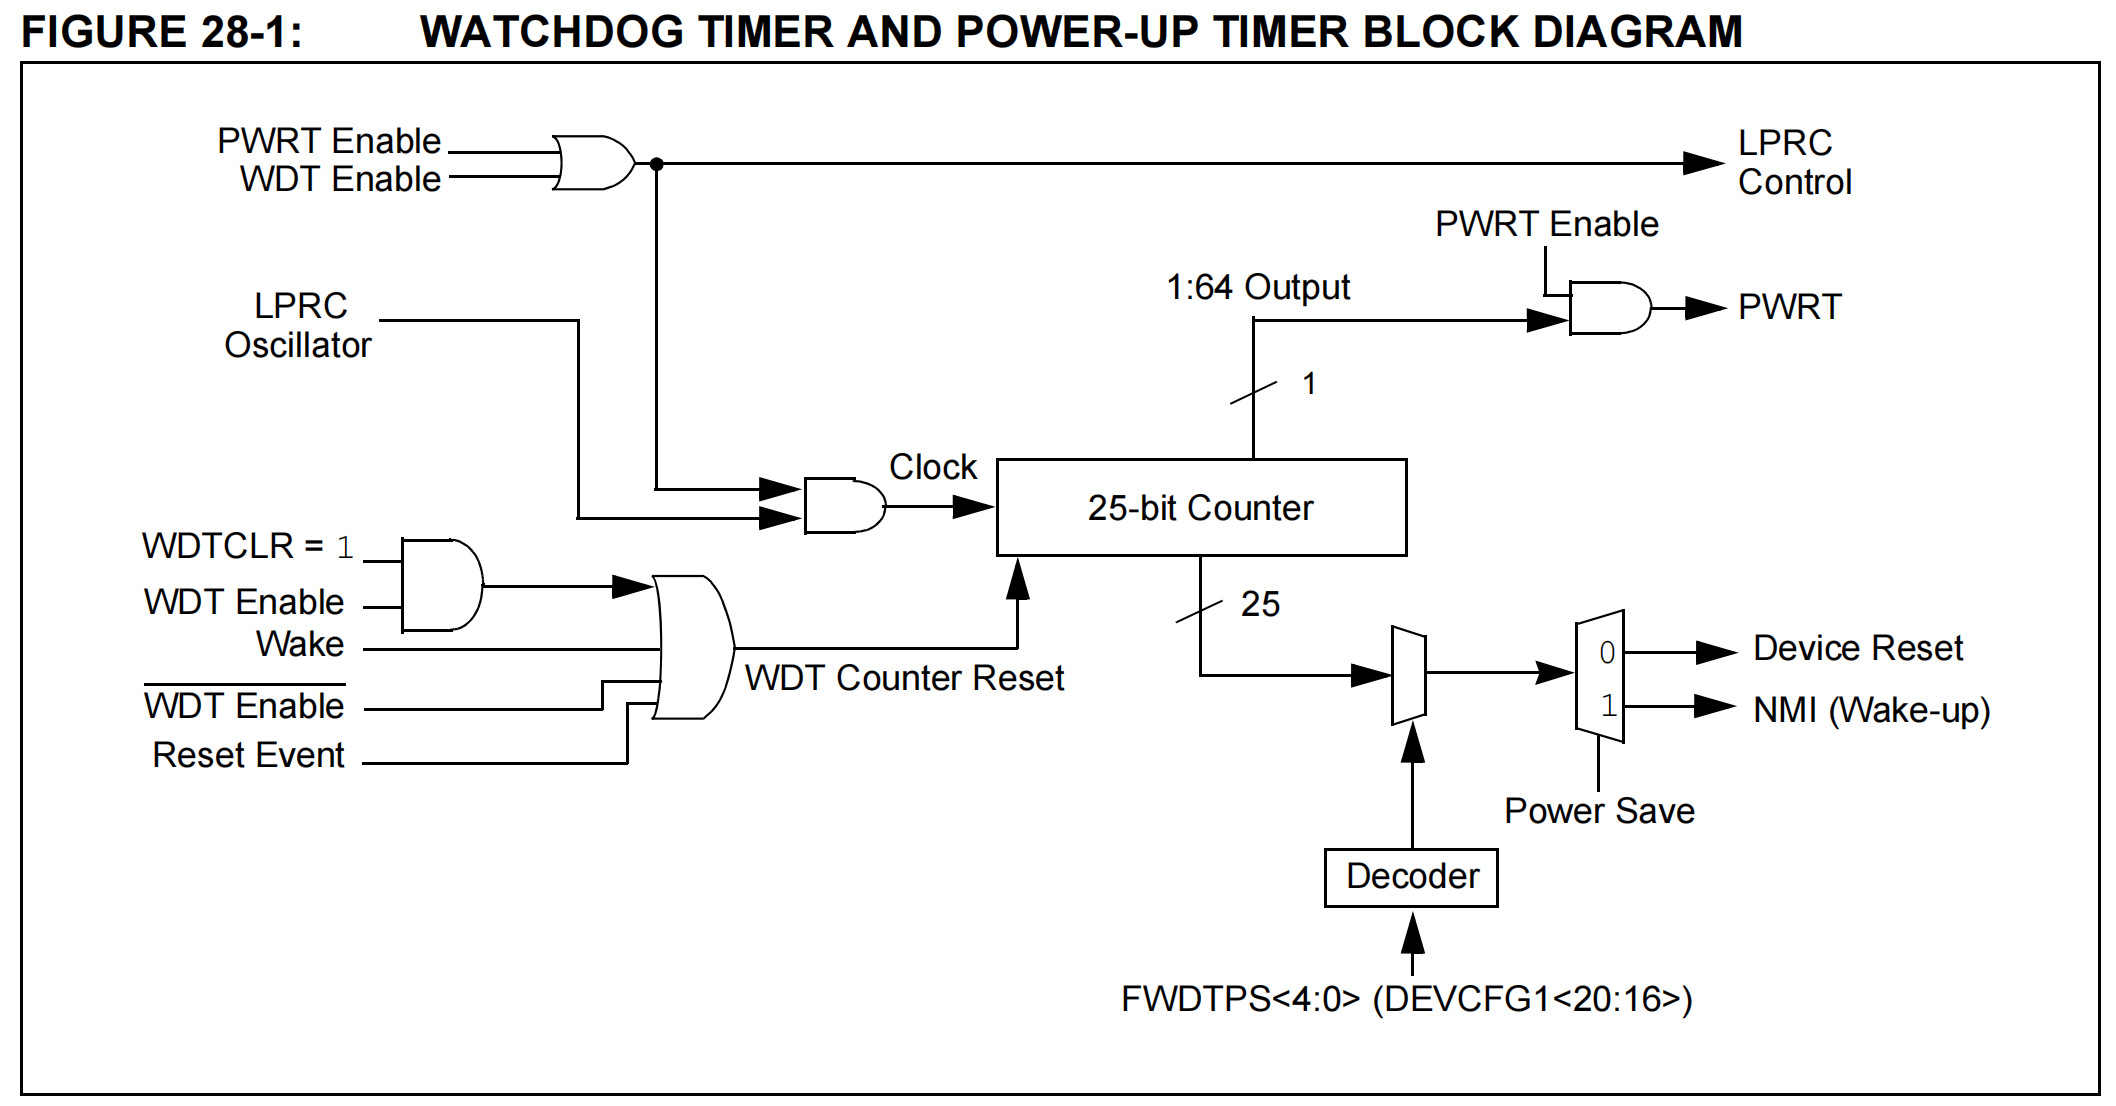
\includegraphics[width=0.8\linewidth]{Watch_dog_timer_block_diagram.png}
            \label{fig:Watch_dog_timer_block_diagram.png}
          \end{figure}

          \par Also used to check software malfunction. Error if software not periodically clear WDT
      \end{itemize}

  \end{enumerate}


\section*{L8 --- Input Capture}
  \par The Input Capture module is useful in applications requiring frequency (period) and pulse measurement.


  \begin{enumerate}[label = \arabic*.]
    \item \textbf{Advantage (comparing to naive solution)}
      \begin{enumerate}[label = \arabic*.]
        \item Accurate
        \item No preemption issue
        \item Don't bother CPU too much
      \end{enumerate}

    \item \textbf{Block diagram}
      \begin{figure}[H]
        \centering
        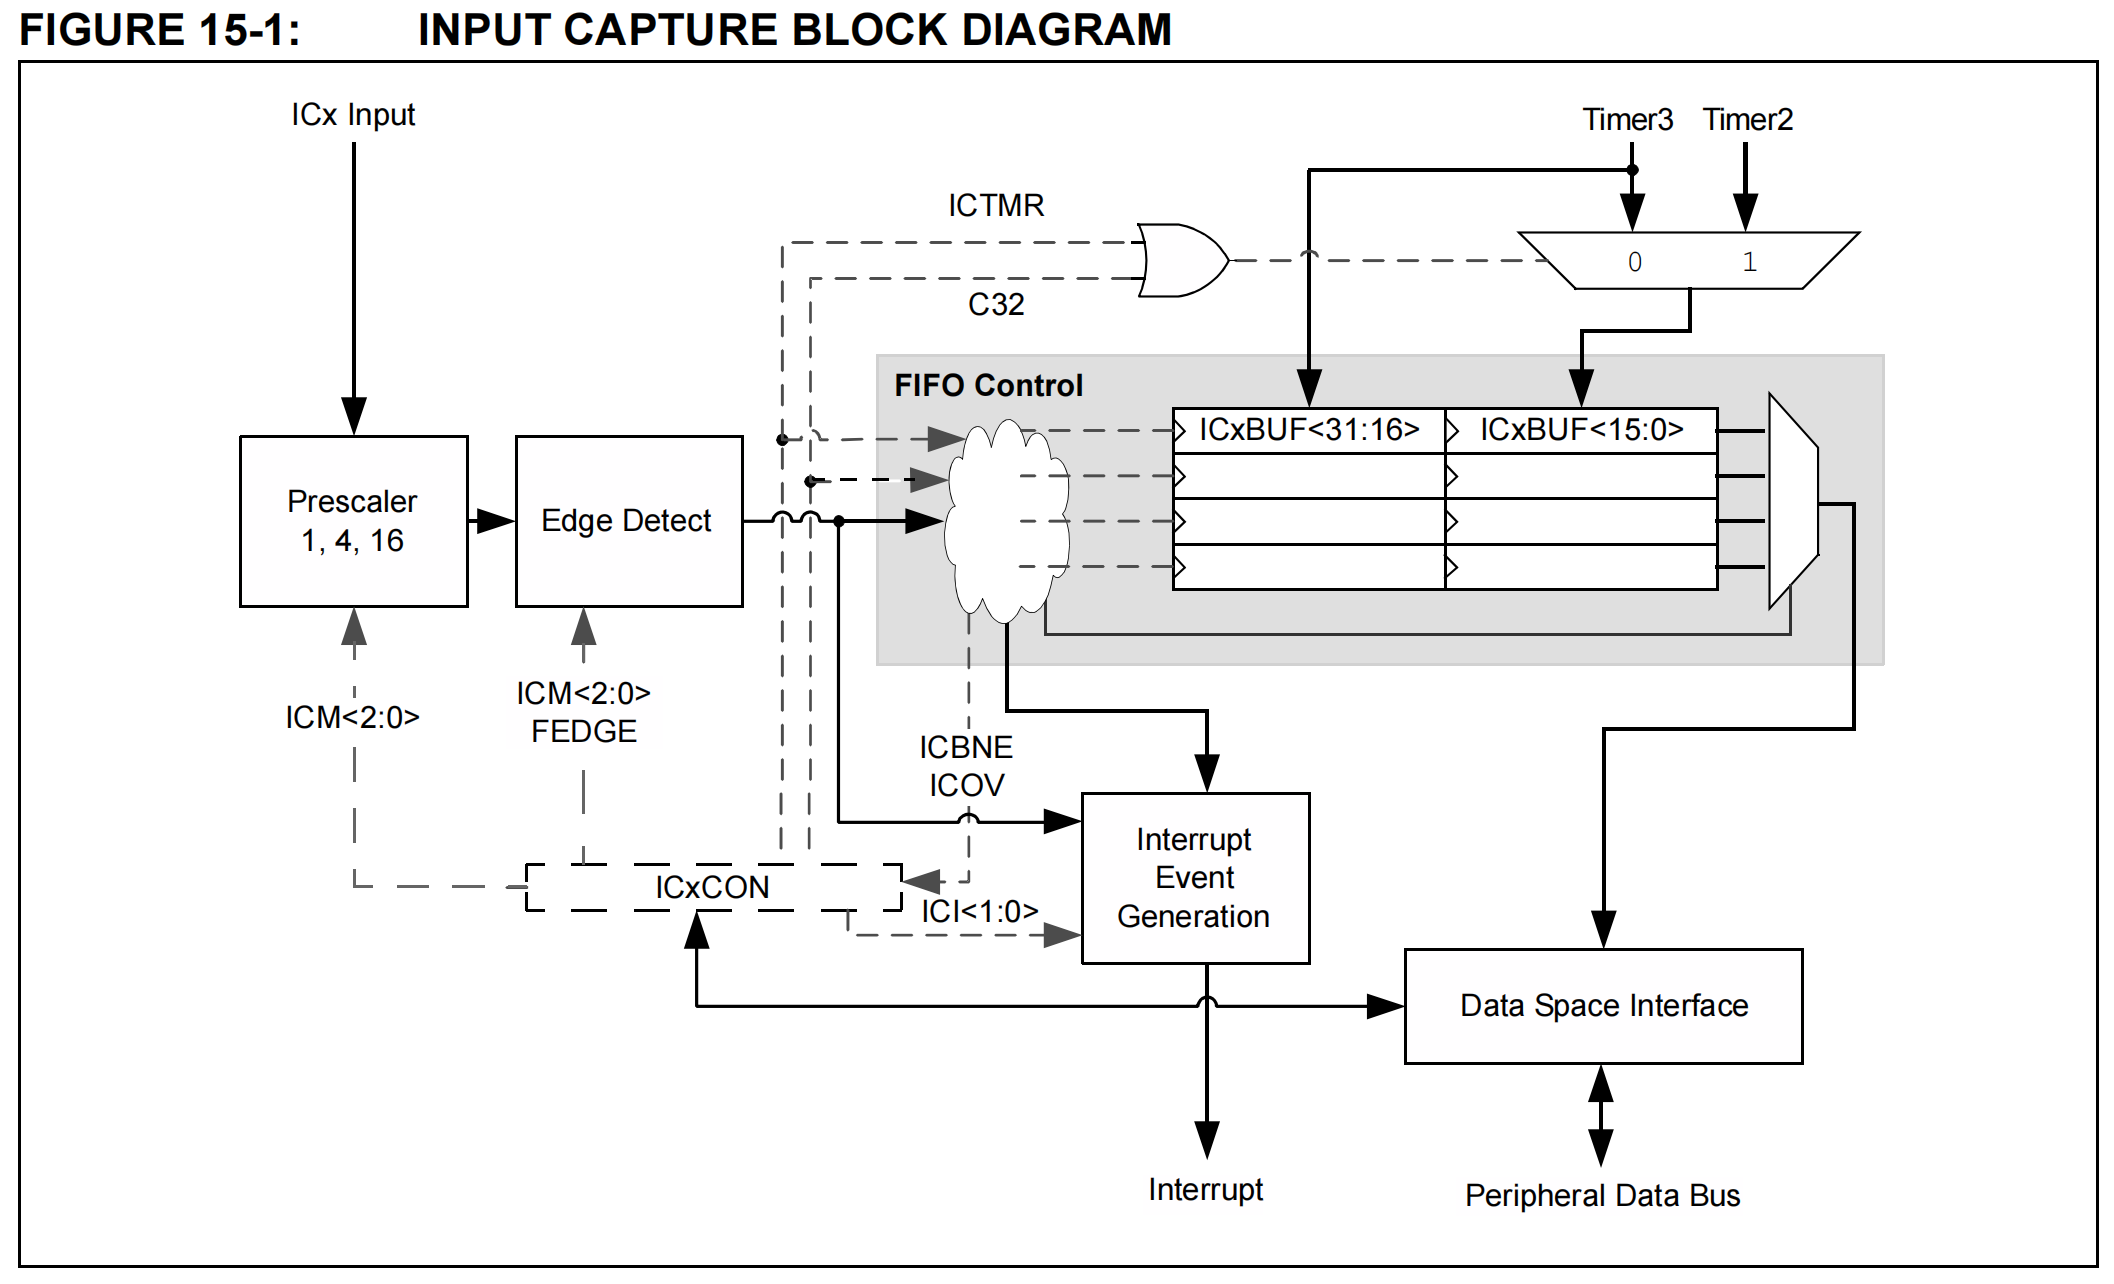
\includegraphics[width=0.9\linewidth]{Input_capture_block_diagram.png}
        \label{fig:Input_capture_block_diagram.png}
      \end{figure}

    \item \textbf{Operation modes}
      \begin{itemize}[leftmargin = 1cm]
        \item Simple capture event modes
          \begin{itemize}[leftmargin = 1cm]
            \item Capture timer value on every falling edge
            \item Capture timer value on every rising edge
            \item Capture timer value on every edge, with specified starting edge (rising or falling)
          \end{itemize}
        \item Prescaled capture event modes
          \begin{itemize}[leftmargin = 1cm]
            \item Capture timer value on every 4th rising edge
            \item Capture timer value on every 16th rising edge
          \end{itemize}
        \item Edge detect mode
        \item Interrupt-only mode
      \end{itemize}

    \item \textbf{Persistent interrupt}
      \par Interrupt is not cleared unless the interrupt condition is cleared.
      \begin{figure}[H]
        \centering
        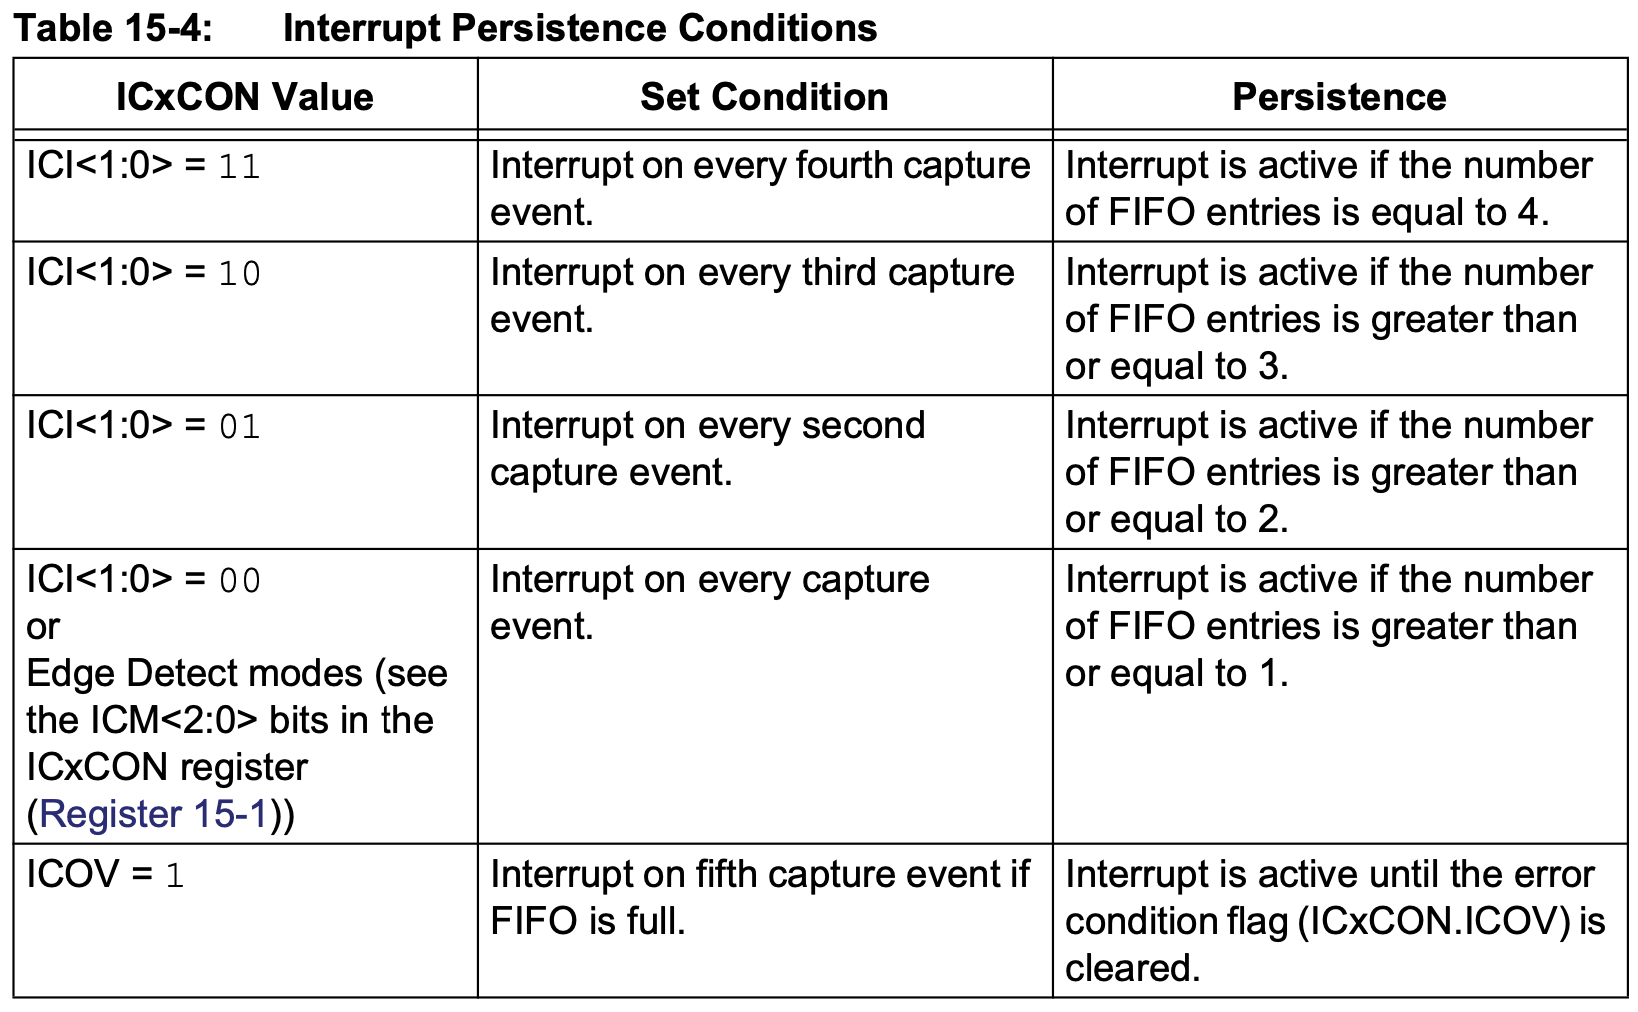
\includegraphics[width=0.6\linewidth]{Input_capture_persistent_condition.png}
        \label{fig:Input_capture_persistent_condition.png}
      \end{figure}

    \item \textbf{Simple capture event modes}
      \begin{itemize}[leftmargin = 1cm]
        \item 2--3 \( T_{PB} \) delay after the event due to synchronization
        \item Capture input is sampled by \verb|PBCLK|, therefore input signal high and low width \( >T_{PB} \).
      \end{itemize}

    \item \textbf{Edge Detect Mode}
      \begin{itemize}[leftmargin = 1cm]
        \item Prescaler and interrupt count not used.
        \item Buffer overflow never signals.
        \item Interrupt request on every capture.
      \end{itemize}

    \item \textbf{Interrupt-only mode}
      \begin{itemize}[leftmargin = 1cm]
        \item Rising edge on ICx triggers an interrupt
          \begin{itemize}[leftmargin = 1cm]
            \item Not functioning during normal operation
            \item No timer capture
            \item No buffer update
          \end{itemize}
        \item Used only as a wake-up mechanism for SLEEP or IDLE modes
      \end{itemize}

    \item \textbf{Capture buffer flags}
      \begin{itemize}[leftmargin = 1cm]
        \item \verb|ICBNE| (\verb|ICxCON<3>|): IC buffer not empty
          \begin{itemize}[leftmargin = 1cm]
            \item Read-only
            \item Signals when 1 or more entries
          \end{itemize}
        \item \verb|ICOV| (\verb|ICxCON<4>|): IC buffer overflow
          \begin{itemize}[leftmargin = 1cm]
            \item Signals on the 5th capture
            \item All extra capture values are lost, until flag cleared
            \item Flag cleared when
              \begin{itemize}[leftmargin = 1cm]
                \item IC Module disabled
                \item Module reset
                \item \verb|ICBNE| becomes 0 --- IC buffer empty
              \end{itemize}
          \end{itemize}
      \end{itemize}


    \item \textbf{Capture event and interrupt event}
      \begin{itemize}[leftmargin = 1cm]
        \item Capture event: capture change of \verb|ICx| and store timer value in the FIFO\@.
        \item Interrupt event: interrupt after certain amount of capture events.
      \end{itemize}

    \item \textbf{Examples}
      \par See reference manual or slides.
  \end{enumerate}


\section*{L9 --- Output Compare and PWM}
  \par The Output Compare module is used to generate a single pulse or a series of pulses in response to selected time base events.
  \begin{enumerate}[label = \arabic*.]
    \item \textbf{Block diagram}
      \begin{figure}[H]
        \centering
        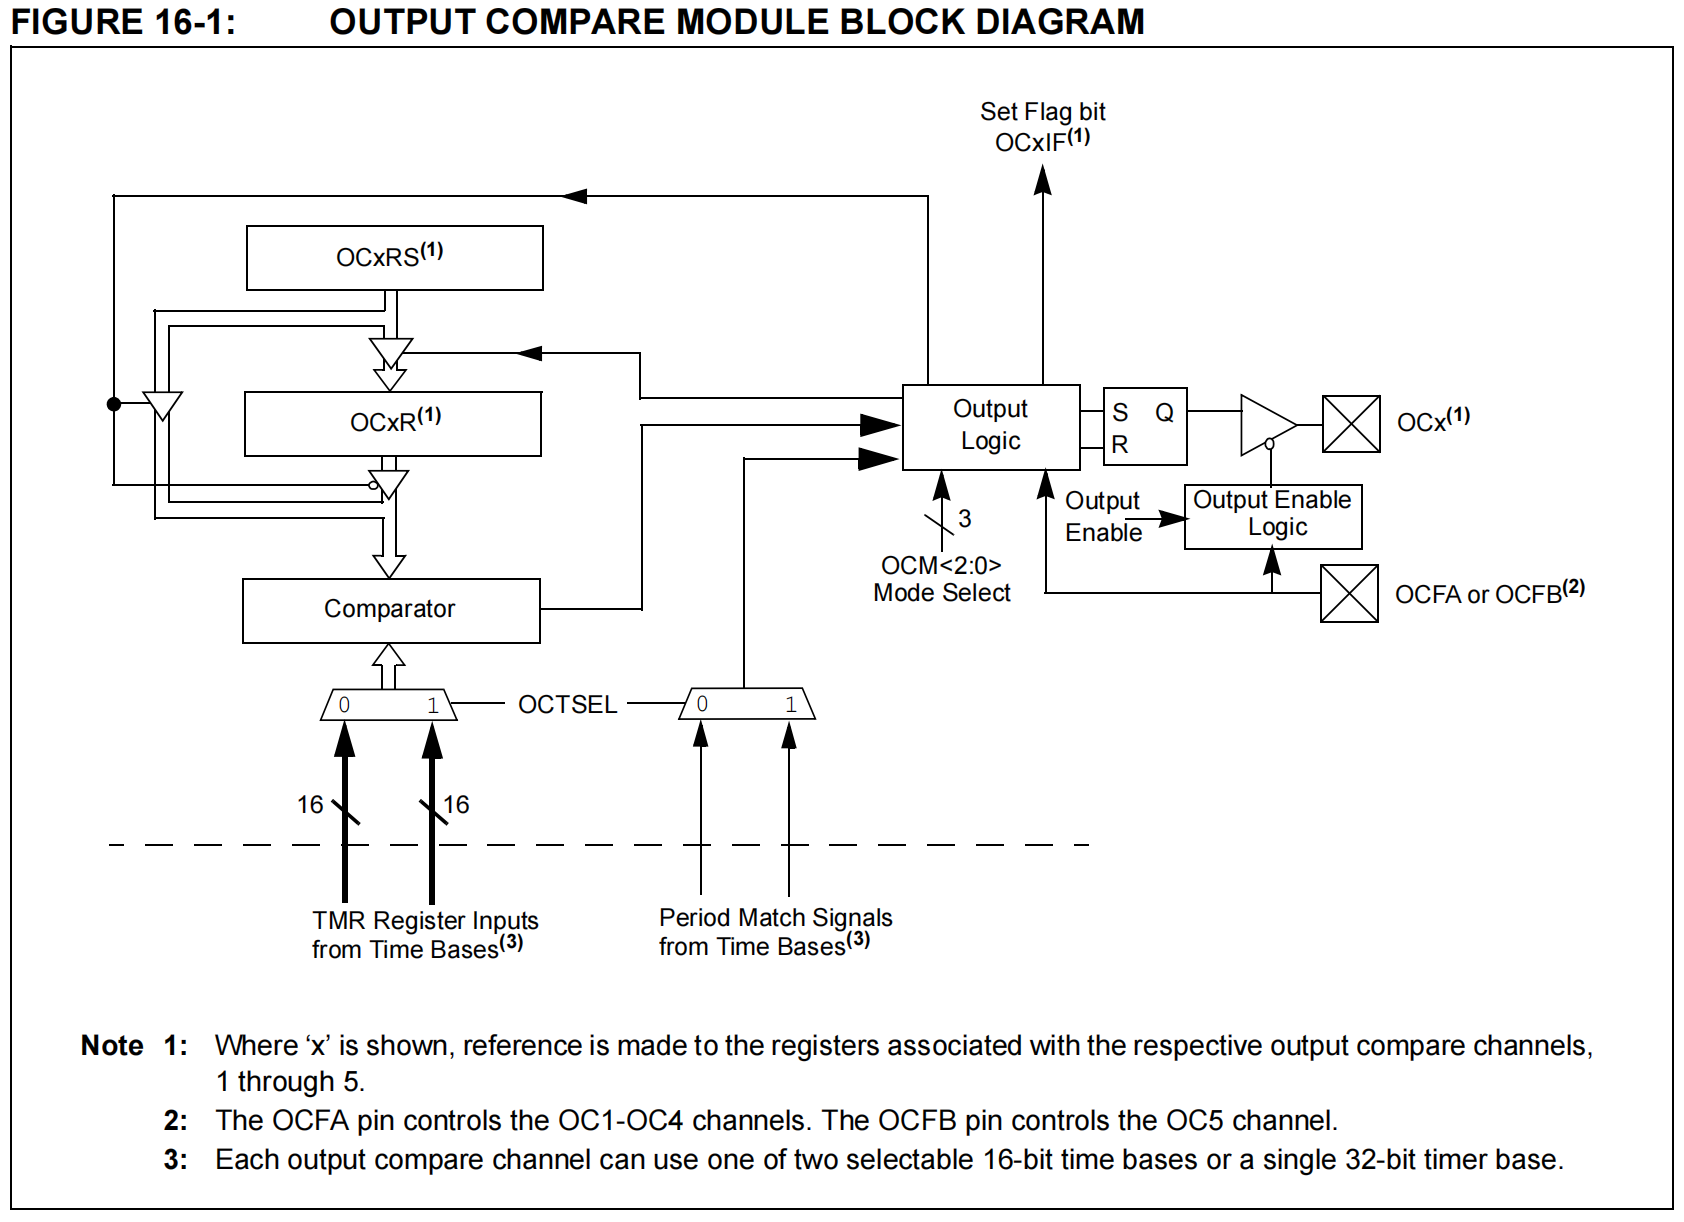
\includegraphics[width=0.9\linewidth]{Output_compare_block_diagram.png}
        \label{fig:Output_compare_block_diagram.png}
      \end{figure}

    \item \textbf{Operation mode}
      \begin{itemize}[leftmargin = 1cm]
        \item Single Compare Match mode
          \par Drive high, drive low, toggle
        \item Dual Compare Match mode
          \par Single output pulse, continuous output pulses
        \item Simple Pulse Width Modulation (PWM) mode
          \par With or without fault protection input
      \end{itemize}

    \item \textbf{Single Compare Match mode}
      \begin{itemize}[leftmargin = 1cm]
        \item Compare forces \verb|OCx| pin high; initial state of pin is low. Interrupt is generated on the single compare match event.
        \item Compare forces \verb|OCx| pin low; initial state of pin is high. Interrupt is generated on the single compare match event.
        \item Compare toggles \verb|OCx| pin. Toggle event is continuous and an interrupt is generated for each toggle event.
      \end{itemize}

    \item \textbf{Dual Compare Match mode}
      \par Single or continues pulse.

    \item \textbf{Single pulse special situations}
      \begin{itemize}[leftmargin = 1cm]
        \item \verb|PRy >= OCxRS > OCxR = TMRy = 0|
          \par The initial match of \verb|OCxR| and \verb|TMRy| at 0 doesn't drive high, work normally afterwards
        \item \verb|PRy >= OCxR >= OCxRS|
          \par Match \verb|OCxR| first, match \verb|OCxRS| in next counting round
        \item \verb|OCxRS > PRy >= OCxR|
          \par Only rising edge generated on first match, then signal remains high, no interrupt generated
        \item \verb|OCxR > PRy|
          \par Not working, \verb|OCx| remains low
      \end{itemize}

    \item \textbf{PWM Signal (Pulse-width modulation)}
      \par Information is encoded into the signal width.
      \begin{itemize}[leftmargin = 1cm]
        \item Advantages of PWM
          \begin{itemize}[leftmargin = 1cm]
            \item Average value proportional to duty cycle
            \item Low power used in transistors used to switch the signal
            \item Fast switching possible due to MOSFETS and power transistors at speeds in excess of 100 kHz
            \item \textbf{Digital signal is resistant to noise less}
            \item Heat dissipated versus using resistors for intermediate voltage values
          \end{itemize}
        \item Disadvantages of PWM
          \begin{itemize}[leftmargin = 1cm]
            \item Cost Complexity of circuit
            \item Radio Frequency Interference
            \item Voltage spikes
            \item Electromagnetic noise
          \end{itemize}
      \end{itemize}

    \item \textbf{PWM Operation Mode}
      \par In PWM mode, the \verb|OCxR| register is a \textbf{read-only} slave duty cycle register and \verb|OCxRS| is a buffer register that is written by the user to update the PWM duty cycle.

      \begin{figure}[H]
        \centering
        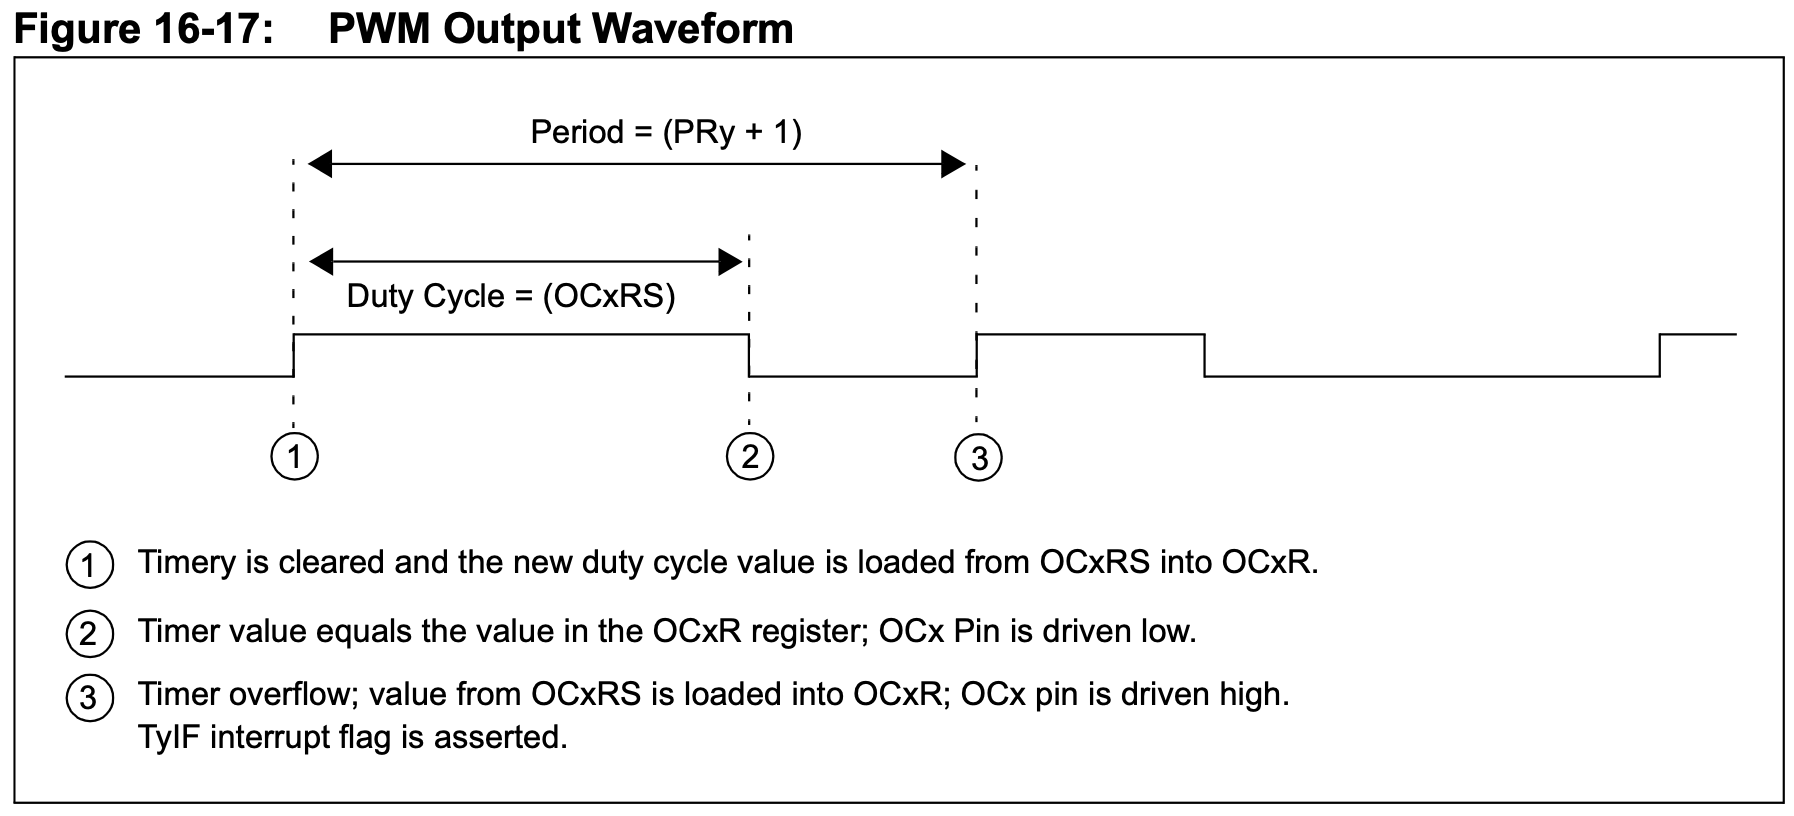
\includegraphics[width=0.8\linewidth]{PWM_output_waveform.png}
        \label{fig:PWM_output_waveform.png}
      \end{figure}

    \item \textbf{Calculations}
      \begin{equation*}
        \begin{aligned}
          T_{\text{PWM}}                      & = (PR + 1) \times T_{\text{PB}}  \times \text{Timer Prescale Value}                                \\
          2^{\text{PWMResolution}}            & = \frac{T_{\text{PWM}}}{T_{\text{timer}} }                                                         \\
          \text{PWMResolution} \text{ (bits)} & = \log_2 \left( \dfrac{F_{\text{PB}} }{F_{\text{PWM}} \times \text{Timer Prescale Value}}  \right) \\
        \end{aligned}
      \end{equation*}

    \item \textbf{Configuration}
      \begin{enumerate}[label = \arabic*.]
        \item Set the PWM period by writing to the selected timer period register (\verb|PRy|).
        \item Set the PWM duty cycle by writing to the \verb|OCxRS| register.
        \item \cprotect\textbf{Write the \verb|OCxR| register with the initial duty cycle.}
        \item Enable interrupts, if required, for the timer and Output Compare modules. The output compare interrupt is required for PWM Fault pin utilization.
        \item Configure the Output Compare module for one of two PWM Operation modes by writing to the Output Compare mode bits, \verb|OCM<2:0>| (\verb|OCxCON<2:0>|).
        \item Set the \verb|TMRy| prescale value and enable the time base by setting \verb|TON| (\verb|TxCON<15>|)\verb| = 1|.
      \end{enumerate}
  \end{enumerate}

\end{document}
